% Template for the submittion to:
%   Statistical Science                 [sts] 
%
%Author: In this template, the places where you need to add information
%        (or delete line) are indicated by {???}.  Mostly the information
%        required is obvious, but some explanations are given in lines starting
%Author:
%All other lines should be ignored.  After editing, there should be
%no instances of ??? after this line.

% use option [preprint] to remove info line at bottom
\documentclass[sts,preprint]{imsart}

\usepackage[right, pagewise]{lineno}
\linenumbers

\usepackage{amsthm,amsmath}
\RequirePackage[colorlinks,citecolor=blue,urlcolor=blue]{hyperref}

% put your definitions there:
\startlocaldefs
\usepackage{amsfonts}
%\usepackage{setspace}
\usepackage{amssymb}
%\usepackage{amsthm}
%\usepackage{graphicx}
%\usepackage{amsmath}
\usepackage{subcaption}
%\setcounter{MaxMatrixCols}{30}
%\usepackage{eps2pdf}
\usepackage{suffix}
\usepackage{color}
\usepackage{bigstrut}
\usepackage{graphicx}
\usepackage{wrapfig}
\usepackage{epstopdf}
%\usepackage{subcaption}
\usepackage{multirow}
\usepackage{nicefrac}
\usepackage[normalem]{ulem}
\usepackage[inline]{enumitem}

% set inline enumerations to use roman numbering
\setlist*[enumerate]{label=(\roman*)}

% this order is important
%\usepackage{hyperref}
%\RequirePackage[colorlinks,citecolor=blue,urlcolor=blue]{hyperref} %IMS
\usepackage{natbib}

%\arxiv{1502.00560}
%\renewcommand{\baselinestretch}{1.5}
%\allowdisplaybreaks

%
% Math commands by Thomas Minka
%
% Revised by Jyotishka Datta & Brandon Willard
%
% TODO: should/could we put includes for dependencies in here?
%
\usepackage{suffix}

\numberwithin{equation}{section}
\newcommand{\var}{{\rm var}}
\newcommand{\Tr}{^{\rm T}}
\newcommand{\rmlog}{\rm log}
\newcommand{\vtrans}[2]{{#1}^{(#2)}}
\newcommand{\kron}{\otimes}
\newcommand{\schur}[2]{({#1} | {#2})}
\newcommand{\schurdet}[2]{\left| ({#1} | {#2}) \right|}
\newcommand{\had}{\circ}
\newcommand{\diag}{{\rm diag}}
\newcommand{\invdiag}{\diag^{-1}}
\newcommand{\rank}{{\rm rank}}
% careful: ``null'' is already a latex command
\newcommand{\nullsp}{{\rm null}}
\newcommand{\tr}{{\rm tr}}
\renewcommand{\vec}{{\rm vec}}
\newcommand{\vech}{{\rm vech}}
\renewcommand{\det}[1]{\left| #1 \right|}
\newcommand{\pdet}[1]{\left| #1 \right|_{+}}
\newcommand{\pinv}[1]{#1^{+}}
\newcommand{\erf}{{\rm erf}}
\newcommand{\hypergeom}[2]{{}_{#1}F_{#2}}

% boldface characters
\renewcommand{\a}{{\bf a}}
\renewcommand{\b}{{\bf b}}
\renewcommand{\c}{{\bf c}}
\renewcommand{\d}{{\rm d}}  % for derivatives
\newcommand{\e}{{\bf e}}
\newcommand{\f}{{\bf f}}
\newcommand{\g}{{\bf g}}
\newcommand{\h}{{\bf h}}
%\newcommand{\k}{{\bf k}}
% in Latex2e this must be renewcommand
\renewcommand{\k}{{\bf k}}
\newcommand{\m}{{\bf m}}
\newcommand{\n}{{\bf n}}
%\renewcommand{\o}{{\bf o}}
\newcommand{\p}{{\bf p}}
%\newcommand{\q}{{\bf q}}
\renewcommand{\r}{{\bf r}}
\newcommand{\s}{{\bf s}}
\renewcommand{\t}{{\bf t}}
\renewcommand{\u}{{\bf u}}
%\renewcommand{\v}{{\bf v}}
\newcommand{\w}{{\bf w}}
\newcommand{\x}{{\bf x}}
\newcommand{\y}{{\bf y}}
%\newcommand{\z}{{\bf z}}
\newcommand{\A}{{\bf A}}
\newcommand{\B}{{\bf B}}
\newcommand{\C}{{\bf C}}
\newcommand{\D}{{\bf D}}
\newcommand{\E}{\mathbb E}
\newcommand{\F}{{\bf F}}
\newcommand{\G}{{\bf G}}
\renewcommand{\H}{{\bf H}}
\newcommand{\I}{{\bf I}}
\newcommand{\J}{{\bf J}}
\newcommand{\K}{{\bf K}}
\renewcommand{\L}{{\bf L}}
\newcommand{\M}{{\bf M}}
\newcommand{\Nor}{{\cal N}}  % for normal density
%\newcommand{\N}{{\bf N}}
\renewcommand{\O}{{\bf O}}
\renewcommand{\P}{\mathbb P}
\newcommand{\Q}{{\bf Q}}
\newcommand{\R}{{\bf R}}
%\renewcommand{\S}{{\bf S}}
\newcommand{\T}{{\bf T}}
\newcommand{\U}{{\bf U}}
\newcommand{\V}{\mathbb V}
\newcommand{\W}{{\bf W}}
\newcommand{\X}{{\bf X}}
\newcommand{\Y}{{\bf Y}}
\newcommand{\Z}{{\bf Z}}

% this is for latex 2.09
% unfortunately, the result is slanted - use Latex2e instead
%\newcommand{\bfLambda}{\mbox{\boldmath$\Lambda$}}
% this is for Latex2e
\newcommand{\bfLambda}{\boldsymbol{\Lambda}}

% Yuan Qi's boldsymbol
\newcommand{\bsigma}{\boldsymbol{\sigma}}
\newcommand{\balpha}{\boldsymbol{\alpha}}
\newcommand{\bpsi}{\boldsymbol{\psi}}
\newcommand{\bphi}{\boldsymbol{\phi}}
\newcommand{\bbeta}{\boldsymbol{\beta}}
%\newcommand{\Beta}{\boldsymbol{\eta}}
\newcommand{\btau}{\boldsymbol{\tau}}
\newcommand{\bvarphi}{\boldsymbol{\varphi}}
\newcommand{\bzeta}{\boldsymbol{\zeta}}
\newcommand{\bnabla}{\boldsymbol{\nabla}}
\newcommand{\blambda}{\boldsymbol{\lambda}}
\newcommand{\bLambda}{\boldsymbol{\Lambda}}

\newcommand{\btheta}{\boldsymbol{\theta}}
\newcommand{\bpi}{\boldsymbol{\pi}}
\newcommand{\bPi}{\boldsymbol{\Pi}}
\newcommand{\bxi}{\boldsymbol{\xi}}
\newcommand{\bSigma}{\boldsymbol{\Sigma}}

\newcommand{\bgamma}{\boldsymbol{\gamma}}
\newcommand{\bGamma}{\boldsymbol{\Gamma}}

\newcommand{\bmu}{\boldsymbol{\mu}}
\newcommand{\bnu}{\boldsymbol{\nu}}
\newcommand{\bPsi}{\boldsymbol{\Psi}}
\newcommand{\bepsilon}{\boldsymbol{\epsilon}}
\newcommand{\bOmega}{\boldsymbol{\Omega}}

\newcommand{\1}{{\bf 1}}
\newcommand{\0}{{\bf 0}}

%\newcommand{\comment}[1]{}

\newcommand{\bs}{\backslash}

 \newcommand{\notS}{{\backslash S}}
 \newcommand{\nots}{{\backslash s}}
 \newcommand{\noti}{{\backslash i}}
 \newcommand{\notj}{{\backslash j}}
 \newcommand{\nott}{\backslash t}
 \newcommand{\notone}{{\backslash 1}}
 \newcommand{\nottp}{\backslash t+1}
% \newcommand{\notz}{\backslash z}

\newcommand{\notk}{{^{\backslash k}}}
%\newcommand{\noti}{{^{\backslash i}}}
\newcommand{\notij}{{^{\backslash i,j}}}
\newcommand{\notg}{{^{\backslash g}}}
\newcommand{\wnoti}{{_{\w}^{\backslash i}}}
\newcommand{\wnotg}{{_{\w}^{\backslash g}}}
\newcommand{\vnotij}{{_{\v}^{\backslash i,j}}}
\newcommand{\vnotg}{{_{\v}^{\backslash g}}}
\newcommand{\half}{\frac{1}{2}}
\newcommand{\quart}{\frac{1}{4}}
\newcommand{\msgb}{m_{t \leftarrow t+1}}
\newcommand{\msgf}{m_{t \rightarrow t+1}}
\newcommand{\msgfp}{m_{t-1 \rightarrow t}}

\newcommand{\proj}[1]{{\rm proj}\negmedspace\left[#1\right]}
\newcommand{\argmin}{\operatornamewithlimits{argmin}}
\newcommand{\argmax}{\operatornamewithlimits{argmax}}

\newcommand{\dif}{\mathrm{d}}
\newcommand{\abs}[1]{\lvert#1\rvert}
\newcommand{\norm}[1]{\lVert#1\rVert}
\newcommand{\vectornorm}[1]{\left|\left|#1\right|\right|}

\newcommand{\rnorm}{\mathcal{N}}
\newcommand{\bx}{{\bf x}}
\newcommand{\ba}{{\bf a}}
\newcommand{\bb}{{\bf b}}
\newcommand{\bc}{{\bf c}}
\newcommand{\bd}{{\bf d}}
\newcommand{\bX}{{\bf X}}
\newcommand{\by}{{\bf y}}
\newcommand{\IG}{\mathcal{IG}}
\newcommand{\dd}[2]{\frac{\partial #1}{\partial #2}}
\newcommand{\lhat}[1][i]{\hat\lambda_{#1}^{-1(g)}}
\newcommand{\what}[1][j]{\hat\omega_{#1}^{-1(g)}}
\newcommand{\bone}{{\bf 1}}
\newcommand{\Li}{\hat\Lambda^{-1(g)}}
\newcommand{\Oi}{\hat\Omega^{-1(g)}}
\newcommand{\iid}{\stackrel{\mathrm{iid}}{\sim}}
\newcommand{\iidp}{\stackrel{\mathrm{P}}{=}}
\newcommand{\iidd}{\stackrel{\mathrm{D}}{=}}
\newcommand{\defeq}{\operatorname{:=}}

% the last {} is a hack for double subscript errors
\newcommand{\estHsp}{\ensuremath{{\hat{\theta}}_{HS+}}{}}
\newcommand{\estHs}{\ensuremath{{\hat{\theta}}_{HS}}{}}
\newcommand{\estJs}{\ensuremath{{\hat{\theta}}_{JS}}{}}
\newcommand{\MSE}{\mathrm{MSE}}
%
% Meijer-G additions
%
\DeclarePairedDelimiterX\MeijerM[3]{\lparen}{\rparen}%
{\begin{smallmatrix}#1 \\ #2\end{smallmatrix}\delimsize\vert\,#3}

\newcommand\MeijerG[8][]{%
  G^{\,#2,#3}_{#4,#5}\MeijerM[#1]{#6}{#7}{#8}}

\WithSuffix\newcommand\MeijerG*[7]{G^{\,#1,#2}_{#3,#4}\MeijerM*{#5}{#6}{#7}}
% end Meijer-G

%
% Generalized Hypergeometric Function (pFq)
%
\DeclarePairedDelimiterX\pFqM[3]{\lparen}{\rparen}%
{\begin{smallmatrix}#1 \\ #2\end{smallmatrix}\delimsize\vert\,#3}

\newcommand\pFq[6][]{%
  {}_{#2}F_{#3}\pFqM[#1]{#4}{#5}{#6}}

\WithSuffix\newcommand\pFq*[5]{{}_{#1}F_{#2}\pFqM*{#3}{#4}{#5}}
% end pFq

\newtheorem{theorem}{THEOREM}
\numberwithin{theorem}{section}
\newtheorem{Proof}{PROOF}
\newtheorem{Def}{DEFINITION}
\numberwithin{Def}{section}
\newtheorem{remark}{REMARK}
\numberwithin{remark}{section}
\newtheorem{Qes}{Question}
\newtheorem{proposition}{PROPOSITION}
\numberwithin{proposition}{section}
\newtheorem{lemma}{LEMMA}
\numberwithin{lemma}{section}
\newtheorem{Cor}{COROLLARY}
\numberwithin{Cor}{section}
\newtheorem{Exa}{Example}
\newtheorem{Eq}{Equation}
\newtheorem{assn}{ASSUMPTION}
%\newtheorem{result}[theorem]{Result}
\newtheorem{result}[theorem]{RESULT}

\usepackage{booktabs,array}
\def\Midrule{\midrule[\heavyrulewidth]}
\newcount\rowc

\makeatletter
\def\ttabular{%
\hbox\bgroup
\let\\\cr
\def\rulea{\ifnum\rowc=\@ne \hrule height 1.0pt \fi}
\def\ruleb{
\ifnum\rowc=1\hrule height 1.0pt  \else
%\ifnum\rowc=3\hrule height 0.0pt%\heavyrulewidth 
\ifnum\rowc= 3  \hrule height 0.5pt \else%\heavyrulewidth 
\ifnum\rowc= 5  \hrule height 0.5pt \else%\heavyrulewidth 
\ifnum\rowc= 7  \hrule height 0.5pt \else%\heavyrulewidth 
\ifnum\rowc= 9  \hrule height 0.5pt \else%\heavyrulewidth 
\ifnum\rowc= 11  \hrule height 0.5pt %\heavyrulewidth 
  \else \hrule height 0pt%\lightrulewidth
\fi\fi\fi\fi\fi\fi}
\valign\bgroup
\global\rowc\@ne
\rulea
\hbox to 7em{\strut \hfill##\hfill}%
\ruleb
&&%
\global\advance\rowc\@ne
\hbox to 7em{\strut\hfill##\hfill}%
\ruleb
\cr}
\def\endttabular{%
\crcr\egroup\egroup}


\graphicspath{{./figs/}}

%\theoremstyle{definition}
%\newtheorem{definition}{Definition}
 %
%\theoremstyle{remark}
%\newtheorem{remark}{Remark}
%

%% For compressing some space: 
%\setlength{\textfloatsep}{10pt plus 1.0pt minus 2.0pt}
%\setlength{\floatsep}{12.0pt plus 2.0pt minus 5.0pt}
%\setlength{\intextsep}{12.0pt plus 2.0pt minus 5.0pt}
%\setlength{\belowcaptionskip}{-2pt}

%\setlength{\textwidth}{6.25in}
%\setlength{\textheight}{9.25in}
%%\setlength{\evensidemargin}{0in}
%%\setlength{\oddsidemargin}{0in}
%\setlength{\topmargin}{-.5in}
%%\setlength{\parskip}{.1in}  
%\setlength{\parindent}{0.0in}  
\endlocaldefs

\begin{document}

\begin{frontmatter}

% "Title of the paper"
\title{Lasso Meets Horseshoe: A Survey}
\runtitle{Lasso Meets Horseshoe}

% indicate corresponding author with \corref{}
% \author{\fnms{John} \snm{Smith}\corref{}\ead[label=e1]{smith@foo.com}\thanksref{t1}}
% \thankstext{t1}{Thanks to somebody} 
% \address{line 1\\ line 2\\ printead{e1}}
% \affiliation{Some University}

\author{\fnms{Anindya} \snm{Bhadra}\ead[label=e1]{bhadra@purdue.edu}}
\address{250 N. University St., West Lafayette, IN 47907. \printead{e1}}
\vspace{-0.1in}
\affiliation{Purdue University}
%\and
\author{\fnms{Jyotishka} \snm{Datta} \corref{} \ead[label=e2]{jd033@uark.edu}}
\address{1 University of Arkansas, Fayetteville, AR 72704. \printead{e2}}
\affiliation{University of Arkansas}
%\and
\author{\fnms{Nicholas G.} \snm{Polson}\ead[label=e3]{ngp@chicagobooth.edu}}
\address{5807 S. Woodlawn Ave., Chicago, IL 60637. \printead{e3}}
\affiliation{University of Chicago  \\   Booth School of Business}
%\and
\author{\fnms{Brandon} \snm{Willard}\ead[label=e4]{bwillard@uchicago.edu}}
\address{5807 S. Woodlawn Ave., Chicago, IL 60637. \printead{e4}}
\affiliation{University of Chicago  \\   Booth School of Business}


\runauthor{Bhadra, Datta, Polson and Willard}

\begin{abstract}
The goal of this paper is to contrast and survey the major advances in two of the most commonly used high-dimensional techniques, namely, the Lasso and horseshoe regularization. Lasso is a gold standard for predictor selection while horseshoe is a state-of-the-art Bayesian estimator for sparse signals. Lasso is fast and scalable and uses convex optimization whilst the horseshoe is non-convex.  Our novel perspective focuses on three aspects: 
\begin{enumerate*}
  \item theoretical optimality in high dimensional inference for the Gaussian
    sparse model and beyond, 
  \item efficiency and scalability of computation and 
  \item methodological development and performance. 
\end{enumerate*}. 
\end{abstract}

\begin{keyword}[class=MSC]
\kwd[Primary ]{62J07, 62J05}
\kwd{sparsity}
\kwd{regression} \kwd{sparsity}, \kwd{regression}, \kwd{Lasso}, \kwd{global-local priors}, \kwd{horseshoe}, \kwd{horseshoe+}, \kwd{regularization}, \kwd{hyper-parameter tuning}.
\kwd[; secondary ]{62H15, 62F03}
\end{keyword}

%\begin{keyword}
%\kwd{}
%\kwd{}
%\end{keyword}

\end{frontmatter}

\section{Introduction}

High-dimensional predictor selection and sparse signal recovery are routine statistical and machine learning practice. 
There is a vast growing literature for both Classical and Bayesian computation of large scale inference problems. Whilst this area is 
too large review here, we revisit two popular sparse parameter estimation techniques, the Lasso \citep{tibshirani96} and the horseshoe 
estimator \citep{carvalho2010horseshoe}. Specifically, we focus on three areas: performance in high-dimensional data, theoretical 
optimality and computational efficiency. 

Sparsity and ultra-sparsity rely on the property of a few large signals among many (nearly) zero noisy observations. 
A common goal in high dimensional inference is to recover the low-dimensional signals observed in noisy observations. 
This problem encompasses four related areas: 

\begin{enumerate}
  \item Estimation of the underlying sparse parameter vector. 
  \item Multiple testing where the \# tests is much larger than the sample size, $n$. 
  \item Regression subset selection where \# of covariates $p$ is far larger than $n$. 
	\item Out-of-sample prediction. 
\end{enumerate}

There are a rich variety of methodologies for high-dimensional regularization which implicitly or explicitly penalize model
 dimensionality. Lasso (Least Absolute Shrinkage and Selection Operator) produces a sparse estimate by constraining the $\ell_1$ 
norm of the parameter vector. Lasso's widespread popularity is due to a multitude of factors, in particular its computational 
efficiency of Least Angle Regression method \citep{efron_least_2004} and simple coordinate descent approaches of 
\citet{friedman_pathwise_2007}, and its ability to produce a sparse solution, with optimality (oracle) properties for both estimation 
and variable selection \citep[\textit{vide}][]{buhlmann2011statistics, james2013introduction, hastie2015statistical}. 
Table~\ref{tab:lasso:ext}, adapted from \citet{tibshirani2014praise},  gives a list of popular regularization methods based on Lasso.
\par 


% Table generated by Excel2LaTeX from sheet 'Sheet1'
\begin{table}[ht!]
  \centering
  \caption{Lasso regularization methods}
  \footnotesize{
    \begin{tabular}{|c|c|}
    \hline
    Method  & Authors  \bigstrut\\
    \hline
    Adaptive Lasso & \citet{zou2006adaptive} \bigstrut[t]\\
    Compressive sensing  & \citet{donoho2006compressed,candes2008restricted} \\
    Dantzig selector  & \citet{candes2007dantzig} \\
    Elastic net & \citet{zou2005regularization} \\
    Fused Lasso & \citet{tibshirani_sparsity_2005} \\
    Generalized Lasso & \citet{tibshirani2011solution} \\
    Graphical Lasso & \citet{friedman2008sparse} \\
    Grouped Lasso & \citet{yuan2006model} \\
    Hierarchical interaction models & \citet{bien_lasso_2013} \\
    Matrix completion & \citet{candes2010power,mazumder2010spectral} \\
    Multivariate methods & \citet{jolliffe2003modified,witten2009penalized} \\
    Near-isotonic regression & \citet{tibshirani2011nearly} \\
    Square Root Lasso  & \citet{belloni2011square} \\
    Scaled Lasso & \citet{sun2012scaled} \\
    Minimum concave penalty & \citet{zhang2010nearly} \\
    SparseNet & \citet{mazumder2012} \bigstrut[b]\\
    \hline
    \end{tabular}%
    }
  \label{tab:lasso:ext}%
\end{table}%

Bayes procedures, on the other hand, can be classified into two categories: discrete mixtures or two-groups model or spike-and-slab priors \citep{johnstone2004needles,efron2010large,efron2008microarrays,bogdan2011asymptotic} and shrinkage priors \citep{bhadra2015horseshoe+,armagan2011generalized,armagan2013generalized,carvalho2009handling,carvalho2010horseshoe,griffin2005alternative,polson2010shrink,castillo2012needles}. {The first class, spike-and-slab prior places a discrete mixture of a point mass at zero (the spike) and an absolutely continuous density (the slab) on each parameter}. The second entails placing absolutely continuous shrinkage priors on the entire parameter vector, that shrink the entire coefficient towards zero. Table \ref{tab:one-gps} provides a sampling of a few continuous shrinkage prior popular in the literature. Both these approaches have their own advantages and caveats, which we discuss in turn.  A key duality being that a penalized approach can be interpreted as Bayesian mode of the posterior distribution under an appropriate shrinkage prior \citep{polson2015mixtures}. 


% Table generated by Excel2LaTeX from sheet 'Sheet1'
\begin{table}[htbp]
  \centering
  \caption{A catalog of Horseshoe and GL shrinkage priors}
  \footnotesize{
    \begin{tabular}{|c|c|}
    \hline
    Global-local shrinkage prior  & Authors  \bigstrut\\
    \hline
    Normal Exponential Gamma & \citet{griffin2005alternative} \bigstrut[t]\\
    Horseshoe & \citet{carvalho2010horseshoe, carvalho2009handling} \\
    Hypergeometric Inverted Beta & \citet{polson2010large} \\
    Generalized Double Pareto & \citet{armagan2011generalized} \\
    Generalized Beta  & \citet{armagan2013generalized} \\
    Dirichlet-Laplace & \citet{bhattacharya2014dirichlet} \\
    Horseshoe+  & \citet{bhadra2015horseshoe+} \\
    Horseshoe-like & \citet{bhadra2017horseshoe} \\
    Spike-and-Slab Lasso & \citet{rovckova2016spike} \\
    R2-D2 & \citet{zhang2016high} \bigstrut[b]\\
		Inverse-Gamma-Gamma & \citet{bai2017inverse} \bigstrut[b]\\
    \hline
    \end{tabular}%
    }
  \label{tab:one-gps}%
\end{table}%


Both Lasso and horseshoe procedures come with strong theoretical guarantees for estimation, prediction and variable selection. {Both procedures possess asymptotic Oracle properties, i.e. identify the true non-zero coefficients as well as achieve the optimal estimation rate.} The behavior of the Lasso estimator in terms of the risk properties has been studied in depth and has resulted in many methods aiming to improve certain features (see Table \ref{tab:lasso:ext}). The horseshoe has been shown to achieve oracle properties in variable selection \citep{datta2013asymptotic} and near-minimaxity in estimation \citep{van2017adaptive} and improved prediction performance in linear regression \citep{bhadra2016prediction}, although theoretical studies of the horseshoe is still an active area. 

%Ultra-sparse signal detection provides a challenge for developing statistical estimators. 
%\subsection{Nearly black normal means model: minimax rate in estimation and optimal rate in testing}

The rest of the paper is organized as follows: Section \ref{sec:2} provides historical background for the normal means (a.k.a the Gaussian compound decision problem) and the sparse regression problems. Section \ref{sec:3} provides the link between regularization and an optimization perspective viewed through a probabilistic Bayesian lens. Section \ref{sec:stat-prop} compares and contrasts the statistical risk properties of Lasso and the horseshoe prior. Sections \ref{sec:5} and \ref{sec:horse-comp} discuss the issues of hyper-parameter selection and computational strategies. Section \ref{sec:simulation} provides two simulation experiments comparing horseshoe prior with penalized regression methods for linear model and logistic regression with varying degree of dependence between predictors. We discuss applications of Lasso and the horseshoe in Section \ref{sec:app-ext} and provide directions for future work in Section \ref{sec:9}. 


\section{Sparse Normal Means, Regression and Variable Selection}\label{sec:2}

\subsection{Sparse Normal Means} Suppose that we observe data from the probability model $(y_i \mid \theta_i)  \id \Nor (\theta_i,1)$ for $i = 1, \ldots, n$. Our primary inferential goal is to estimate the vector of normal means $ \btheta = ( \theta_1, \ldots , \theta_n )$ and a secondary goal would be to simultaneously test if $\theta_i$'s are zero or not. We are interested in the sparse paradigm where a large proportion of the parameter
vector contains zeros.  {The `ultra-sparse' \citep{bhadra2015horseshoe+} or `nearly black' \citep{donoho1992maximum} regime occurs when the parameter vector $\theta$ lies in the set $ l_0[ p_n] \equiv \{ \theta : \# ( \theta_i \neq 0 ) \leq p_n \} $ with the upper bound on the number of non-zero parameter values $ p_n = o(n) $ as $ n \to \infty$.}

A natural solution for inference under sparsity is the two-groups model that puts a non-zero probability spike at zero and a suitable prior on the non-zero $\theta_i$'s (\textit{vide} Appendix \ref{sec:2gp}). The inference is then based on the posterior probabilities of non-zero $\theta_i$'s based on the discrete mixture model. The two-groups model possesses a number of frequentist and Bayesian optimality properties. \cite{johnstone2004needles} showed that a thresholding-based
estimator for $\btheta$ under the two-groups model with an empirical Bayes estimate for the sparsity proportion attains the minimax rate in $\ell_q$ norm for $q \in (0,2]$ for $\btheta$ that are either nearly black or belong to an $\ell_p$ ball of `small' radius. \cite{castillo2012needles} treated a full Bayes version of the problem and again found an estimate that is minimax in $\ell_q$ norm for mean vectors that are either nearly black or have bounded weak $\ell_p$ norm for $p \in (0,2]$. 

%We now turn to the problem of variable selection in sparse regression. 

\subsection{Sparse Linear Regression} 

A related inferential problem is high dimensional linear regression with sparsity constraints on the parameter vector $\btheta$. We are interested in the linear regression model:

\[
\Y = \X \btheta + \bepsilon,
\]

where $\X = [\X_1, \cdots, \X_p]$ is a $p \times n$ matrix of predictors and $\bepsilon \sim \Nor(\0, \sigma^2\I_n)$. 

Our focus is on the sparse solution where $p \gg n$ and most of $\theta_i$'s are zero. Similar to the
sparse normal means problem, our goal is to identify the non-zero entries of $\btheta$ as well as estimate it. There are a wide variety of methods based on the penalized likelihood approach that solves the following optimization problem:

\begin{align}
  \min_{\btheta} \sum_{i=1}^{n} &  \left( y_i - \theta_0 - \sum_{j=1}^{p} \theta_j x_{i,j} \right)^2 + \text{pen}_{\lambda}(\btheta), \label{eq:penalize} \\
  \text{where } & \text{pen}_{\lambda}(\btheta) = \sum_{j=1}^{p} p_{\lambda}(\theta_j) \text{ is a separable penalty} \nonumber
\end{align}

Lasso uses an $\ell_1$ penalty, $p_{\lambda}(\theta_j) = -\lambda \abs{\theta_j}$, and simultaneously performs variable selection while maintaining estimation accuracy.  Another notable variant is the best subset selection procedure corresponding to the $\ell_0$ penalty $p_{\lambda}(\theta_j) = -\lambda \1\{\theta_j \ne 0\}$.
There has been a recent emphasis on non-concave separable penalties such as MCP \citep{zhang2010nearly} or SCAD \citep{fan2001variable}, that act as a tool for variable selection and estimation. Penalization methods can be viewed in terms of the posterior modes they imply under an induced prior relating to the penalty in \eqref{eq:penalize}--via $p(\btheta) = -\log \pi(\btheta)$, where $\pi(\cdot)$ is a suitable prior for $\btheta$. We discuss the penalization methods from a Bayesian viewpoint in the next section. 


\subsection{Variable Selection}


Variable or predictor selection is intimately related to high-dimensional sparse linear regression.  A sparse model provides interpretability, computational efficiency, and stability of inference. Lasso's success has inspired many estimation methods that rely on the convexity and sparsity entailed. The `bet on sparsity' principle \citep{hastie_elements_2009} dictates the use of methods favoring sparsity, as no method uniformly dominates when the true model is dense.  

\begin{remark}

The LAVA method by \citet{chernozhukov2017lava} strictly dominates both Lasso and ridge in a `sparse+dense' model. In fact, the LAVA estimator performs as well as Lasso in a sparse regime and as well as ridge \citep{tikhonov1963solution} in a dense regime. This questions the validity of the `bet on sparsity' principle. 
Although there is no exact analogue of LAVA in the Bayesian world, the one-group shrinkage priors share a common philosophy. The horseshoe-type priors are also designed to work when true $\btheta$ has a few large entries and very many small non-zero entries and produces a `non-sparse' estimator, but LAVA, can recover both the dense and sparse components unlike horseshoe.

\end{remark}

A parallel surge of Bayesian methodologies has emerged for sparse regression problems with an underlying variable selection procedure. Hierarchical Bayesian modeling proceeds by selecting a model dimension $s$, selecting a random subset $S$ of dimension $\abs{S} = s$ and a prior $\pi_S$ on $\mathbb{R}^{S}$. The prior can be written as in \cite{castillo2015bayesian}:

\begin{equation}
  (S,\btheta) \mapsto \binom{p}{\abs{S}}^{-1} 
	\pi_p(\abs{S}) \pi_S(\btheta_S)\delta_{0}(\btheta_{S^c}) \label{eq:bayes-hier}
\end{equation}

\noindent Bayesian approaches for sparse linear regression include \citet{george2000variable, George0000, mitchell88, ishwaran2005spike} and more recently \cite{rovckova2016spike}, who introduce the spike-and-slab Lasso prior, where the hierarchical prior on the parameter and model spaces assumes the form:

\begin{equation}
  \pi(\btheta \mid \gamma) = \prod_{i=1}^{p} [\gamma_i \pi_1(\theta_i) +
  (1-\gamma_i) \pi_0(\theta_i)], \quad \gamma \sim p(\cdot), \label{eq:ssl}
\end{equation}

where $\bgamma$ indexes the $2^p$ possible models, and $\pi_0$, $\pi_1$ model the null and non-null $\theta_i$'s respectively using two Laplace priors with different scales. 

%Despite the \textcolor[rgb]{1,0,0}{attractive theoretical properties} outlined above, the discrete indicators in spike-and-slab models give rise to a combinatorial problem. While some posterior point estimates such as the posterior mean or quantiles might be easily computable for spike-and-slab \citep{castillo2012needles, castillo2015bayesian}, exploring the full posterior using Markov chain Monte Carlo (MCMC) is typically more challenging. 

The continuous one-group shrinkage prior takes a different approach: instead of  placing a prior on the model space to yield a sparse estimator, it models the posterior inclusion probabilities $P(\theta_i \ne 0 \mid y_i)$ directly. The continuous shrinkage prior leads to faster computation relative to the spike-and-slab type priors as exploring the full posterior using point mass mixture priors is prohibitive due to a combinatorial complexity of updating the discrete indicators and infeasibility of block updating of model parameters. In comparison, global-local shrinkage priors typically lead to efficient Gibbs sampling scheme based on block-updating the model parameters. We also note that while full posterior sampling remains a computational hurdle for the spike-and-slab prior, point estimates such as posterior mean and posterior quantiles can be obtained using a polynomial-time algorithm as shown by \citet{castillo2012needles}. \citet{rovckova2016spike} discuss the inefficiency of stochastic search algorithms for exploring the posterior even for moderate dimensions and developed a deterministic alternative to quickly find the maximum a-posteriori model. Here \begin{enumerate*}
  \item increasing the efficiency in computation in the spike-and-slab model
    remains an active area of research \citep[see, e.g., ][]{rovckova2016spike}
    and
  \item some complicating factors in the spike-and-slab model, such as a lack of suitable block updates, have fairly easy solutions for their continuous global-local shrinkage counterparts, facilitating posterior exploration. 
\end{enumerate*}

\citet{carvalho2009handling, polson2010shrink, carvalho2010horseshoe, polson2012half} introduced the `global-local' shrinkage priors. Global-local priors adjust to sparsity via global shrinkage, and identify signals by local shrinkage parameters. The global-local shrinkage idea has resulted in many different priors in the recent past, with a varying degree of theoretical and numerical performance. We compare these different priors and introduce a recently proposed family of horseshoe-like priors in \S \ref{sec:one-gp}.   

The estimators resulting from the one-group shrinkage priors are very different from the shrinkage estimator due to \citet{james_estimation_1961}, who showed that maximum likelihood estimators for multivariate normal means are inadmissible beyond two dimensions. The James--Stein estimator is primarily concerned about the total squared error loss, without much regard for the individual estimates. In problems involving observations lying far away on the tails this leads to `over-shrinkage' \citep{carvalho2010horseshoe}. In reality, an ideal signal-recovery procedure should be robust to large signals. 

%polson2010shrink

\section{Lasso and Horseshoe}\label{sec:3}

%Define estimators / compare shrinkage profiles. Asymptotic of finding zeroes. 
%Explain $\phi(\theta)$ for horseshoe etc. 
%\subsection{Bayesian Regularization : A Useful Duality}

Regularization requires the researcher to specify a measure of fit, denoted by $l(\btheta)$ and a penalty function, denoted by $\phi(\theta)$. Probabilistically,  $l(\theta)$ and $\text{pen}_{\lambda}(\btheta)$ correspond to the negative logarithms of the likelihood and prior distribution, respectively.  

Regularization leads to an optimization problem of the form 
\begin{equation}
  \min_{\btheta \in \Re^d}
  \left\{ l(y \mid \btheta) + \text{pen}_{\lambda}(\btheta) \right\}
  \;, 
  \label{eq:reg}
\end{equation}

and the probabilistic approach leads to a Bayesian hierarchical model

\begin{equation}
  p(y \mid \btheta) \propto \exp\{-l(y \mid \btheta)\} \; , \quad \pi_{\lambda}(\btheta)
  \propto \exp\{ -\text{pen}_{\lambda}(\btheta) \}. 
  \label{eq:pen}
\end{equation}

For appropriate $l(y \mid \btheta)$ and $\text{pen}_{\lambda}(\btheta)$, the solution to \eqref{eq:reg} corresponds to the posterior mode of \eqref{eq:pen}, $\hat{\btheta} = \argmax_{\btheta} p(\btheta \mid y)$, where $p(\btheta \mid y)$ denotes the posterior distribution. The properties of the penalty are then induced by those of the prior.  For example, regression with a least squares log-likelihood subject to an $\ell_2$ penalty or Ridge \citep{tikhonov1963solution, hoerl70} corresponds to a Gaussian prior under the same observation distribution, and an $\ell_1$ penalty (Lasso) \citep{tibshirani96} corresponds to a double-exponential prior \citep{park_bayesian_2008}.

One interpretation of Lasso and related $\ell_1$ penalties are methods designed to perform selection, while ridge and related $\ell_2$ based methods perform shrinkage. Selection-based methods such as the Lasso are unstable in many situations, e.g., in presence of multi-collinearity in the design \citep[ch.3]{hastie_elements_2009}. 

Although `shrinkage' and `selection' are closely related, we tend to distinguish between them in the following sense. Shrinkage methods such as the horseshoe prior shrinks towards 0 by thresholding the shrinkage weights that behave like posterior inclusion probabilities $P(\theta_i \neq 0 \mid y_i)$ to achieve variable selection. 
However, the continuous nature of prior on $\theta_i$ ensures a lack of exact zeros $P(\theta_i = 0 
\mid y_i) = 0$, which is preferred over dichotomous models by some practitioners \citep{stephens2009bayesian} as more realistic.  This is unlike the Lasso that performs explicit selection by making some of estimates 0 and producing a true sparse solution. Ultimately, both selection and shrinkage have their advantages and disadvantages. 

%In this sense, the one-group priors mimic Bayesian model averaging \citep{polson2010shrink}, where one achieves better predictive performance by averaging over models supported by data. Several authors \citep{polson2010shrink, polson2012local, datta2015search} have shown empirically horseshoe outperforms Lasso (as well as Bayesian model averaging) in terms of out-of-sample predictive sum-of-squares error. Ridge regression often performs poorly in prediction, specially in $p \gg n$ situation when $\y$ could be strongly correlated with low variance principal components of the design matrix $\X$. This is where horseshoe prior wins as the relative shrinkage need not be monotone in the singular values of $\X$ \citep{bhadra2016prediction}.

\subsection{Lasso Penalty and Prior}\label{sec:lasso}

%The Lasso based estimate of $\btheta$ is the value of $\btheta$ that maximizes the $\ell_1$ penalized log-likelihood, or equivalently, the posterior mode under a component-wise Laplace prior, as given below: 
%
%\begin{equation}
  %(\text{Penalty}): \; \text{pen}_{\lambda}(\btheta) = \lambda \sum_{j = 1}^{p}  \abs{\theta_j} \; \Leftrightarrow \; \pi_{\lambda}(\btheta) = \exp( - \lambda \sum_{j =
  %1}^{p} \abs{\theta_j}) \; (\text{Prior})
%\end{equation}

As discussed before, the classical Lasso-based estimate is same as the posterior mode under component-wise Laplace prior, and the mode inherits the optimal properties of Lasso. For example, the Oracle inequality in \citet[Eq. (2.8), Th. (6.1)]{buhlmann2011statistics} states that with a proper choice of $\lambda$ of order $\sigma \sqrt{\log(p)/n}$, the mean squared prediction error of Lasso is of the same order as if one knew active set $S_0 = \{j : \theta_j^0 \neq 0 \}$), up to $O(\log(p))$ and a compatibility constant $\phi_0^2$. The compatibility (or restricted eigenvalue) constant reflects the compatibility between the design matrix and the $\ell_1$ norm of $\btheta$, and is defined as follows \citep[Eq (6.4)]{buhlmann2011statistics}:


\begin{definition}\label{def:compatibility}[Compatibility Condition:] 
For $S \subset \{1,2,\ldots,p\}$ and $\btheta \in \mathbb{R}^{p}$, let $\btheta_{j,S} \doteq \theta_j 1\{j \in S\} \in \mathbb{R}^{p}$ (with similar notation for $\btheta_{j \in S} \in \mathbb{R}^{\abs{S}}$), and let $\btheta_{-S} = \theta_{S^c}$. Then the compatibility condition is satisfied for the design $\X$ for the true support set $S = \text{supp}(\btheta)$, if letting $s_0 = \abs{S}$,

\[
\frac{1}{n} \vectornorm{\X\btheta}_2^2 \ge \frac{\phi_0^2}{s_0} \vectornorm{\btheta_{S}}_1^2, \; \text{ for all } \; \btheta \in \mathbb{R}^p \; \text{such that} \; \vectornorm{\btheta_S}_1 \le 3 \vectornorm{\btheta_{-S}}_1
\]

The constant $\phi_0^2$ is called the compatibility (or restricted eigenvalue) constant.
\end{definition}

Lasso also exhibits other desirable properties such as computational tractability, consistency of point estimates of $\btheta$ for suitably $\lambda$, and optimality results on variable selection. 


\subsection{Bayesian Lasso and Elastic Net}

{As discussed before, the posterior mean under Bayesian Lasso, the Bayes estimate under squared error loss, will not satisfy the optimality properties of the posterior mode under the double-exponential prior}. Along these lines, \citet{castillo2015bayesian} argue that the Lasso is essentially non-Bayesian, in that the ``\textsl{full posterior distribution is useless for uncertainty quantification, the central idea of Bayesian inference}." \citet{castillo2015bayesian} provide theoretical result that the full Lasso posterior does not contract at the same speed as the posterior mode. 

However, there are a number of caveats related to the use of a double-exponential prior for the general purposes of shrinkage.  An important example is found in how it handles shrinkage for small observations and
robustness to the large ones.  This behavior is described by various authors, including \cite{polson2010shrink,datta2013asymptotic}, and motivates the key properties of global-local priors. Figure~\ref{fig:priorkappa} provides profile plots as a diagnostic of shrinkage behavior for different priors.

For correlated predictors, \cite{zou2005regularization} proposed a family of convex penalties called `elastic net', which is a hybrid between Lasso and ridge. The penalty term is $\sum_{j=1}^{p} \lambda p_{\alpha}(\theta_j)$, where 

\[
p_{\alpha}(\theta_j) = \half (1-\alpha)\theta_j^2 + \alpha \abs{\theta_j}, \quad j = 1, \ldots, p. 
\]

Both Lasso and elastic net facilitate efficient Bayesian computation via a global-local scale mixture representation \citep{bhadra2016global}. The Lasso penalty arises as a Laplace global-local mixture \citep{andrews1974scale}, while the elastic-net regression can be recast as a global-local mixture with a mixing density belonging to the orthant-normal family of distributions
\citep{hans2011elastic}.  The orthant-normal prior on $\theta_i$, given hyper-parameters $\lambda_1$ and $\lambda_2$, has a density function with the following form:

\begin{equation}
  p(\theta_i \mid \lambda_1, \lambda_2)  = 
  \begin{cases} 
   \phi(\theta_i \mid \frac{\lambda_1}{2\lambda_2}, \frac{\sigma^2}{\lambda_2}) / 2\Phi\left(-\frac{\lambda_1}{2\sigma \lambda_2^{1/2} }\right), & \quad \theta_i < 0, \\
   \phi(\theta_i \mid \frac{-\lambda_1}{2\lambda_2}, \frac{\sigma^2}{\lambda_2}) / 2\Phi\left(-\frac{\lambda_1}{2\sigma \lambda_2^{1/2} }\right), & \quad \theta_i \geq 0. \end{cases} 
  \label{eq:hans}
\end{equation}


\subsection{Horseshoe Penalty and Prior}\label{sec:one-gp}

The horseshoe prior is a continuous shrinkage rule for sparse signal recovery. Specifically, the horseshoe prior for $\theta_i$, given a global shrinkage parameter $\tau$, is given by the hierarchical model 

\begin{align}
  (y_i \mid \theta_i) & \sim \Nor(\theta_i , \sigma^2),\;
  (\theta_i \mid \lambda_i, \tau) \sim 
  \Nor(0, \lambda_i^2 \tau^2) \nonumber \\ \lambda_i ^2 &
  \sim \operatorname{C}^{+}(0,1), \quad i = 1, \ldots, n. 
  \label{eq:hs}
\end{align}

As previously noted, the horseshoe prior operates under a different philosophy: that of modeling the inclusion probability directly rather than using a discrete mixture to model sparsity. To see this, note that the posterior mean under the horseshoe prior can be written as a linear function of the observation:

\[
\E(\theta_i \mid y_i) = \{1- \E(\kappa_i \mid y_i) \} y_i \text{ where } \kappa_i = 1/(1+\lambda_i^2 \tau^2)
\]

The name `horseshoe' arises from the shape of the beta prior density of the shrinkage weights, $\kappa_i$. A comparison with the posterior mean obtained under the two-groups model reveals that the shrinkage weights perform the same job as the posterior inclusion probability $P(\theta_i \ne 0 \mid y_i)$ for recovering a sparse signal. Since the shrinkage coefficients are not formal Bayesian posterior quantities, we refer to them as `pseudo posterior inclusion probabilities.'

Consider the normal means model: $y_i \mid \theta_i \sim \Nor(\theta_i,1), \theta_i \mid \lambda_i, \tau \sim \Nor(0, \lambda_i^2 \tau^2)$, $i = 1,2, \ldots, n$. The marginal likelihood after reparametrizing $\kappa_i = (1+\lambda_i^2\tau^2)^{-1}$ is,  $p(y_i \mid \kappa_i, \tau) = \kappa_i^{1/2} \exp \left(-\kappa_i y_i^2/2 \right)$. The posterior density of $\kappa_i$ identifies signals and noises by letting $\kappa_i \to 0$ and $\kappa_i \to 1$ respectively. Since the marginal likelihood puts no probability density on $\kappa_i = 0$, it does not help identify the signals. Intuitively, any prior that drives the probability to either extremities should be a good candidate for sparse signal reconstruction. The horseshoe prior does exactly that: it cancels the $\kappa_i^{1/2}$ term and replaces it with a $(1-\kappa_i)^{-1/2}$ to enable $\kappa_i \to 1$ in the posterior. The horseshoe+ prior \citep{bhadra2015horseshoe+} takes this philosophy one step further, by creating a $U$-shaped Jacobian for transformation from $\lambda_i$ to $\kappa_i$-scale. The double-exponential on the other hand, yields a prior that decays at both ends with a mode near $\kappa_i = 1/4$, thus leading to a posterior that is neither good at adjusting to sparsity, nor at recovering large signals.
 
Figure \ref{fig:priorkappa} plots the posterior density $p(\kappa_i \mid y_i)$ for the horseshoe, horseshoe+, and the Laplace priors. Figure \ref{fig:score} shows the resulting shrinkage function by plotting the input observations against the output estimates for horseshoe, horseshoe+, and Laplace priors, along with the maximum likelihood estimator ($\hat{\btheta} = \y$). Both Lasso and horseshoe shrink the small observations, but while horseshoe and horseshoe+ leave the large inputs unshrunk, Lasso shrinks them by a non-vanishing amount, resulting in a non-zero bias. We also plot the shrinkage function for the post-lava estimator \citep{chernozhukov2017lava} (\textit{vide} Appendix C) which works well on dense+sparse signals, and has the robustness property lacking in Lasso/Laplace prior. 

\begin{figure}[!ht]
%\vspace{-0.2in}
\begin{subfigure}{0.48\linewidth}
\centering
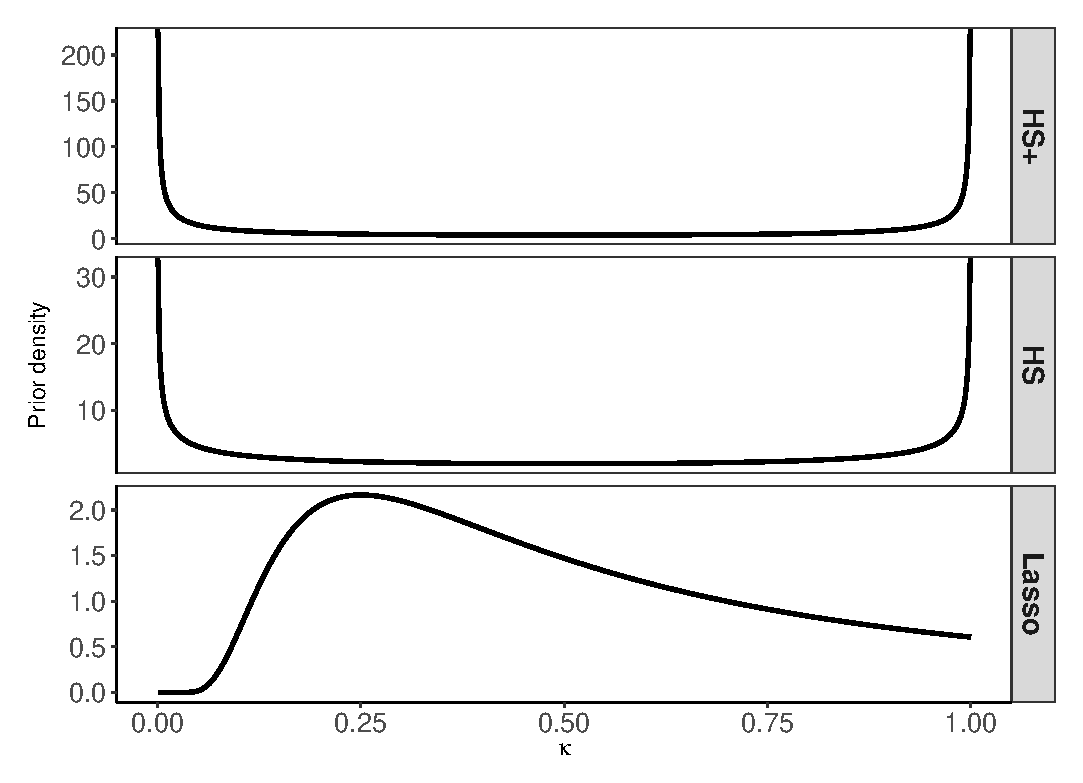
\includegraphics[height = 2in, width=\textwidth]{prior_diff_kappa}
\caption{\footnotesize{Shrinkage factor $\kappa_i$,($p(\kappa_i \mid y_i)$)}}
\label{fig:priorkappa}
\end{subfigure}
\begin{subfigure}{0.48\linewidth}%
\centering
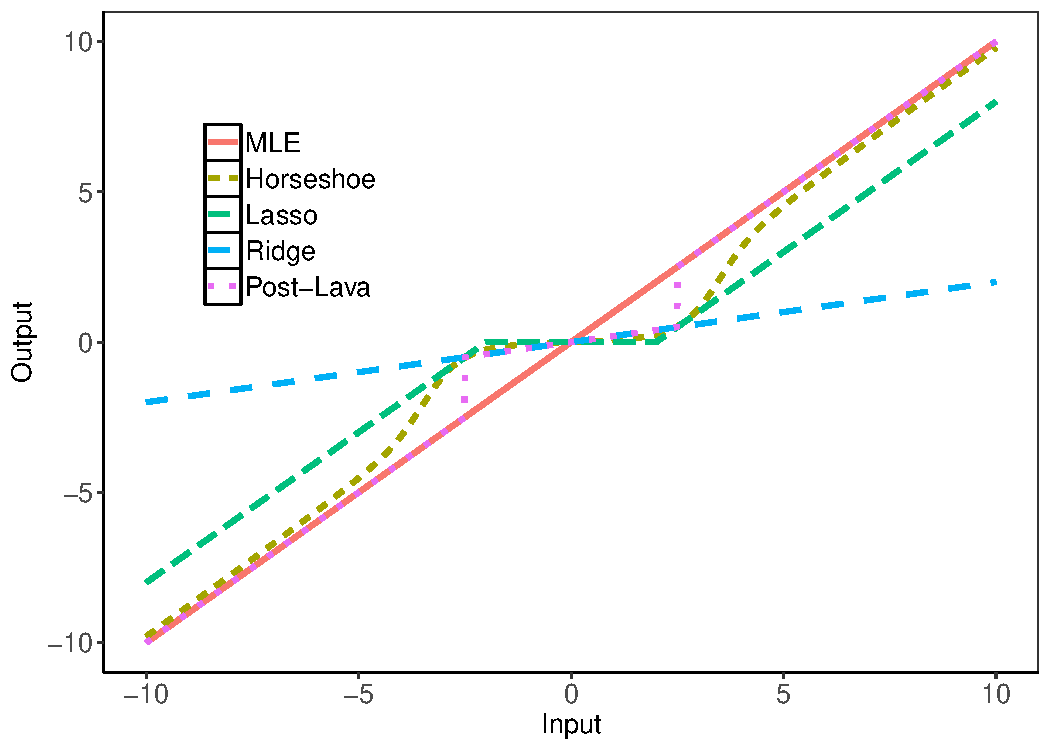
\includegraphics[height = 2in, width=\columnwidth]{shrinakge_hs_lasso_lava}%
\caption{Score function}%
\label{fig:score}%
\end{subfigure}
\label{fig:score-kappa}
\caption{\footnotesize{Posterior density of shrinkage weight for the horseshoe, horseshoe+, and Laplace
prior, where $(1- \kappa_i)$ can be interpreted as the pseudo posterior inclusion probability or $P(\theta_i \ne 0 \mid y_i)$, and (b) shrinkage function for LAVA, Lasso, ridge and the horseshoe estimator. For
LAVA shrinkage function, we have chosen $\lambda_1 = \lambda_l = 4$ and $\lambda_2 = \lambda_r = 4$, and for the horseshoe prior the value of global shrinkage parameter $\tau$ is fixed at $0.1$.}}
\end{figure}


\citet{carvalho2010horseshoe} provided strong numerical evidence that this one-group shrinkage rule approximately behaves like the answers from a two-groups model under sparsity and attains super-efficiency in reconstructing the true density. Although, the main goal of a shrinkage prior is estimation, this interpretation of shrinkage weights as inclusion probabilities led \citet{carvalho2010horseshoe} to propose a multiple testing rule by using a threshold on $1-\hat{\kappa}_i$ values. \citet{datta2013asymptotic}
investigated the theoretical optimality of such a decision rule under a $0$-$1$ additive loss and showed that the horseshoe multiple testing rule attains the Bayes oracle up to a multiplicative constant. 

There are a number of closed-form results for the posterior distribution under a horseshoe prior. Although the prior density under the horseshoe prior doesn't admit a closed form, we can write the horseshoe posterior mean using the Tweedies' formula $\E(\theta \mid y) = y + \dd{\ln m(y)}{y}\sigma^2$, which is also the Bayes adjustment that provides an optimal bias-variance trade-off. For the horseshoe prior, Tweedies' formula yields:

\begin{equation}
  \E(\theta_i \mid y_i, \tau) = y_i \left( 1 - \frac{2\Phi_1(\half, 1,
  \frac{5}{2},\frac{y_i^2}{2\sigma^2}, 1-\frac{1}{\tau^2})}{
  3\Phi_1(\half, 1, \frac{3}{2},\frac{y_i^2}{2\sigma^2}, 1-\frac{1}{\tau^2})} \right)
  \;,
\end{equation}
where $\Phi_1$ is the bivariate confluent hypergeometric function \citep{gordy1998computationally}. A similar formula is available for the posterior variance. This enables one to rapidly calculate the posterior mean estimator under the horseshoe prior via a `plug-in' approach with estimated values of the hyper-parameter $\tau$. In a series of papers, \citet{van2014horseshoe,van2015conditions,van2016many,van2017adaptive} showed that the empirical Bayes posterior mean estimator enjoys  a `near-minimax' rate of estimation if the global shrinkage parameter $\tau$ is chosen suitably. We discuss the statistical properties of horseshoe posterior mean estimator and the induced decision rule in more details in \S~\ref{sec:stat-prop}. 

%
The horseshoe prior is a member of a wider class of global-local scale mixtures of normals that admit following hierarchical form \citep{polson2010shrink}: 

\begin{gather*}
(\y \mid \btheta) \sim \Nor(\btheta, \sigma^2 \I) ;\; \theta_i \sim \Nor(0, \lambda_i^2 \tau^2) \\
\lambda_i^2 \sim \pi(\lambda_i^2) ; \; (\tau,\sigma^2) \sim  \pi(\tau^2,\sigma^2), i = 1, \ldots, n. 
\end{gather*}

These priors are collectively called global-local shrinkage priors in \cite{polson2010shrink}, since they recover signals by a local shrinkage parameter and adapt to sparsity by a global shrinkage parameter. Some of the popular shrinkage priors include the generalized double Pareto (GDP) \citep{armagan2013generalized}, the three-parameter beta \citep{armagan2011generalized}, and the more recent horseshoe+
\citep{bhadra2015horseshoe+} and the Dirichlet--Laplace \citep{bhattacharya2014dirichlet} priors. A natural question is \textit{how do
we compare these priors?} It is known due to several authors \citep[e.g.]{polson2010shrink,bhadra2015default,van2015conditions} that the key features of a global-local shrinkage prior is a peak at origin and heavy tails. An early example of such a prior was proposed by \citet{cutillo2008larger} in the context of wavelet thresholding where a heavier tail was attained by modeling $\theta \sim \Nor(
0, \tau^2)$ and $\tau^2 \sim (\tau^2)^{-k}$ where $k > 1/2$. 
We list a few popular global-local shrinkage priors along with their behavior near origin and the tails on Table \ref{tab:one-gps}. A detailed list of shrinkage priors proposed in the recent past is deferred to \S~\ref{sec:app-ext}.

\begin{table}%
\centering
\begin{tabular}{| c | c |c |}
\hline
Prior & Origin Behavior & Tails \\
\hline 
Horseshoe & $-\log(\abs{\theta})$ & $\abs{\theta}^{-2}$ \\
Horseshoe+ & $-\log(\abs{\theta})$ & $\abs{\theta}^{-1}$ \\
Horseshoe-like & $-\abs{\theta}^{1-\epsilon}\log(\abs{\theta})$ & $\abs{\theta}^{1-\epsilon}$ $\epsilon \ge 0$\\
GDP & Bounded at origin & $\abs{\theta}^{-(\alpha + 1)}, \alpha \ge 0$ \\
$DL_{a}$ ($DL_{\frac{1}{n}}$) & $\abs{\theta}^{a-1}$ ($\abs{\theta}^{\frac{1}{n}-1}$) & $\exp(-b\abs{\theta})$ \\
\hline
\end{tabular}
\caption{Different Priors: Behavior near origin and tails}
\label{tab:priors}
\end{table}

\begin{figure}[ht!]
% \centering 
  \begin{subfigure}{0.45\linewidth}
	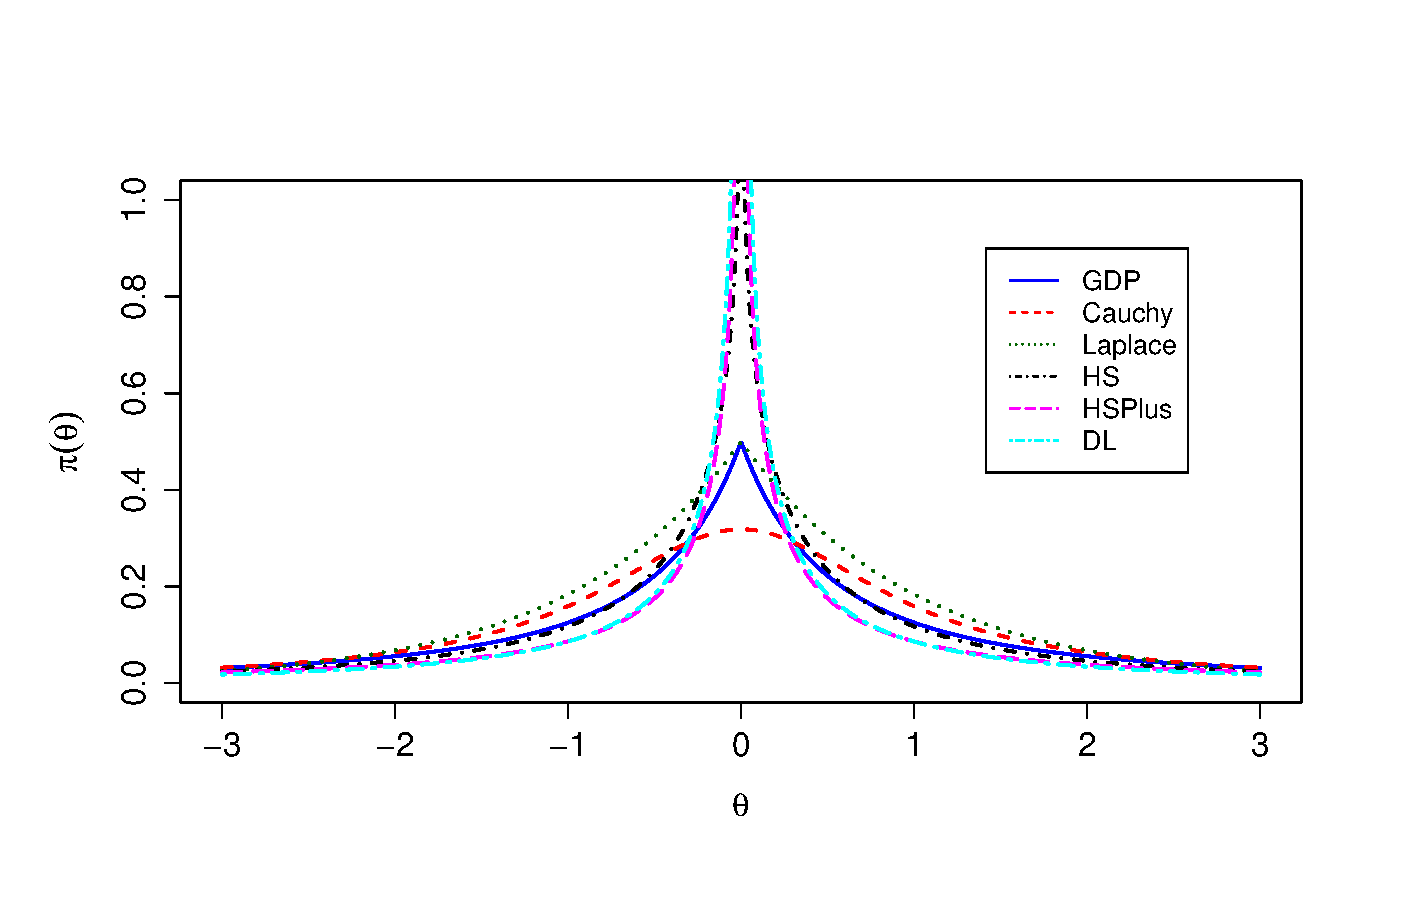
\includegraphics[height=2.5in,width=\textwidth]{densities_zero_new}%
%	\caption{\footnotesize{Marginal prior densities near the origin. The legends denote the horseshoe+ (HSPlus), horseshoe (HS), Dirichlet-Laplace (DL), generalized double Pareto (GDP), Cauchy and Laplace priors.}}
	\label{fig:zero}
	\end{subfigure}
	\hspace{0.1in}
  \begin{subfigure}{0.45\linewidth}
	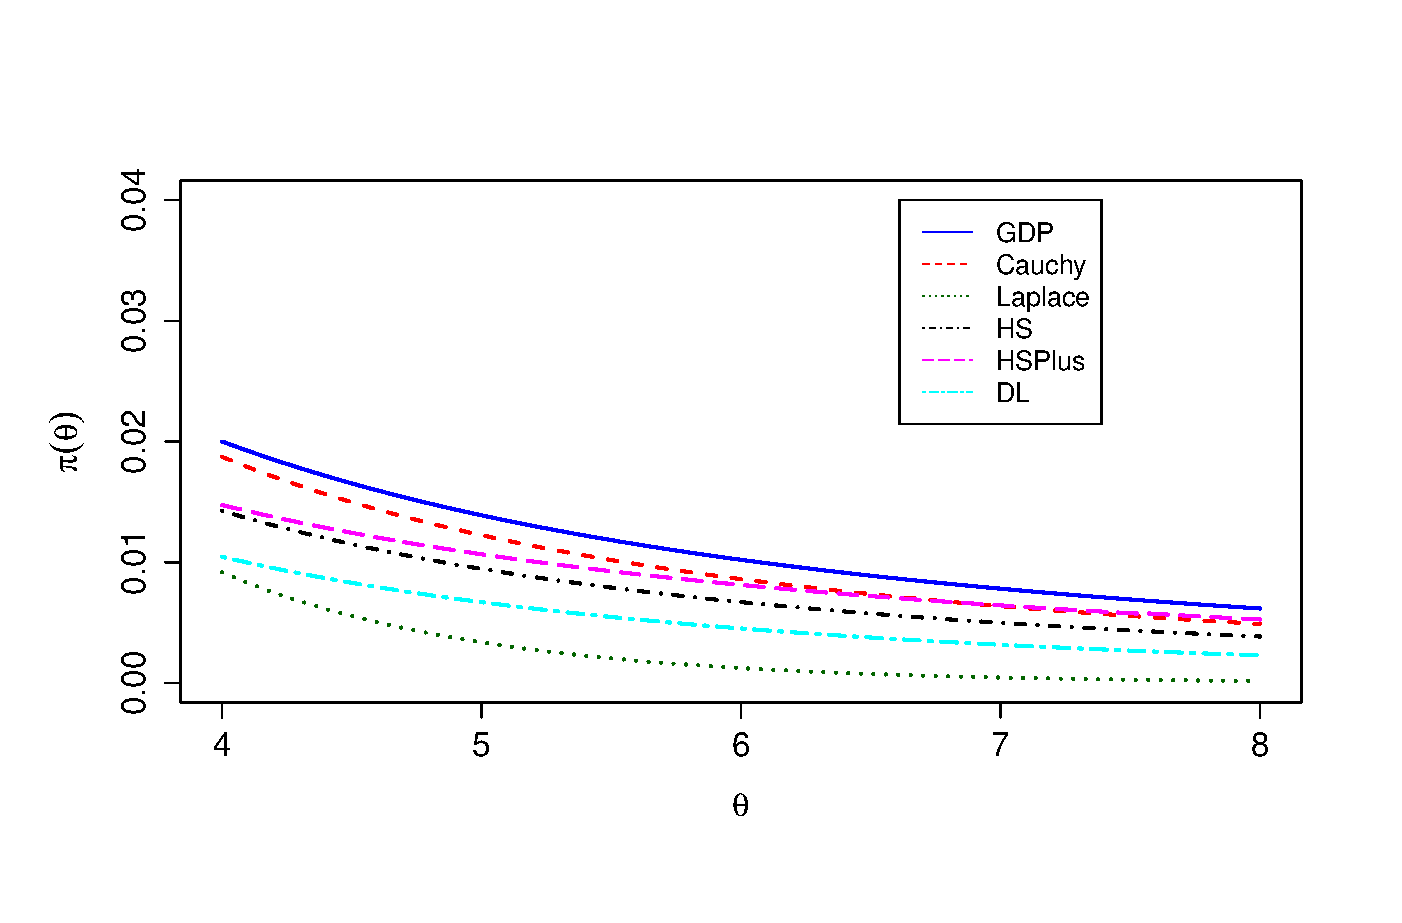
\includegraphics[height=2.5in,width=\textwidth]{densities_tails_new}
  \label{fig:tails}
		\end{subfigure}
 \caption{Marginal prior densities near the origin (left) and in the tail regions (right). The legends denote the horseshoe+ (HSPlus), horseshoe (HS), Dirichlet-Laplace (DL), generalized double Pareto (GDP), Cauchy and Laplace priors.}
\end{figure}

From a regularization view-point, one way to judge a prior is by the penalty it imposes on a likelihood \eqref{eq:reg}, although in a strict Bayesian spirit, a prior should be evaluated based on the whole posterior as shown by several authors including \citep{castillo2015bayesian, van2017adaptive}. %
Although the horseshoe prior leads to optimal performance as a shrinkage prior, the induced penalty $\log \pi(\theta)$ does not admit a closed form as the marginal prior $\pi(\theta)$ is not analytically tractable. This poses a hindrance in learning via Expectation-Maximization or other similar algorithms.  The generalized double Pareto prior of
\citet{armagan2011generalized} admits a closed form solution, but it does not have an infinite spike near zero needed for sparse recovery. Motivated by this fact, \citet{bhadra2017horseshoe} recently proposed the `horseshoe-like' prior by normalizing the tight bounds for the horseshoe prior. Thus, the horseshoe-like
prior attains a unique status within its class: it has a closed form marginal prior for $\theta$, yet with a spike at origin and heavy tails and more importantly, admits a global-local scale mixture representation. The scale mixture representation supports both a traditional MCMC sampling for uncertainty
quantification in full Bayes inference and EM/MM or proximal learning when computational efficiency is the primary concern. 

Since the aim of designing a sparsity prior is achieving higher spike near zero while maintaining regularly varying tails, a useful strategy is to split the range of the prior into disjoint intervals: $[0,1)$ and $[1, \infty)$, and aim for higher spike in one and heavier tail in the other. This leads to a class of `horseshoe-like' priors with more flexibility in shape than any single shrinkage prior. We provide the
general form of horseshoe-like priors and a key representation theorem.  The proof that horseshoe-like prior is a scale mixture with Slash normal mixing density involves Frullani's probabilistic identity \citep[\textit{vide}][pages 406-407]{jeffreys1972methods}, and to save substantial additional space we refer the readers to the proof in \S 5, Lemma 5.1 and Proposition 5.1 of \citet{bhadra2017horseshoe}.

\begin{description}
  \item[Horseshoe-like priors] 
    \citet{bhadra2017horseshoe} have the following marginal prior density for
    $\theta_i$: 
    \begin{equation}
      \tilde p_{\tilde{HS}} (\theta_i \mid \tau^2) = \frac{1}{2 \pi{\tau}}\log
      \left ( 1 + \frac{\tau^2}{\theta_i^2} \right ), \quad  \; \theta_i  \in
      \mathbb{R},\; \tau > 0. \label{eq:hslike}
    \end{equation}
    The general family of horseshoe-like priors can be constructed as a density
    split into disjoint intervals as follows:
    \begin{align}
      p_{hs}(\theta_i \mid \tau^2)&  \propto \begin{cases}
        \frac{1}{\theta_i^{1-\epsilon}}\log \left( 1 + \frac{\tau^2}{\theta_i^2}
          \right) & \text{ if } {\abs{\theta_i} < 1} \\ \theta_i^{1-\epsilon}
          \log \left( 1 + \frac{\tau^2}{\theta_i^2} \right) & \text{ if
        }{\abs{\theta_i} \ge 1}, \\ \end{cases} \; \epsilon \ge 0,\tau > 0.
        \label{eq:split} 
    \end{align}
  \item[Normal scale mixture] 
    The horseshoe-like prior \eqref{eq:hslike} is a Gaussian scale mixture with  a Slash Normal mixing density, which is in turn another Gaussian scale mixture of $\operatorname{Pareto}(1/2)$ density, yielding the following representation theorem: 
    \begin{theorem}[\citet{bhadra2017horseshoe}]\label{th:hslike}
      The horseshoe-like prior in \eqref{eq:hslike} has the following global-local scale mixture representation:
      \begin{equation}
        \begin{gathered}
    (\theta_i \mid t_i, \tau) \sim \Nor\left(0, \frac{\tau^2}{t_i^2} \right),\quad (t_i \mid s_i) \sim \Nor\left(0, s_i \right),\\
          s_i \sim \operatorname{Pareto}\left( \frac{1}{2} \right), \quad t_i \in \mathbb{R}, \; \tau \ge 0.
        \end{gathered}\label{eq:pareto}
      \end{equation}
    \end{theorem}
\end{description}

\begin{table}[!ht]
\centering
%\def~{\hphantom{0}}
\caption{Priors for $\lambda_i$ and $\kappa_i$ for a few popular shrinkage rules}
%{\footnotesize
\begin{tabular}{ccc}
\hline
Prior for $\theta_i$ & Prior for $\lambda_i$ & Prior for $\kappa_i$ \\ 
\hline \\
%GDP & $\frac{\sqrt{2}}{(\lambda_i^2)} \int_{0}^{\infty} \exp \bigg(\sqrt{\frac{2u}{\lambda_i^2}} - u \bigg) \sqrt{u} \mathrm{d}u$  & $\frac{1}{2(1-\kappa)^2} \left[ \frac{\sqrt{\pi} \exp \left\{ \frac{\kappa}{2(1-\kappa)} \right\} Erfc \left\{ \sqrt{\frac{\kappa}{2(1-\kappa)}} \right\}  }{\sqrt{2\kappa(1-\kappa)}} - 1 \right]$ \\[20pt]
Horseshoe & $2/ \left\{ \pi \tau (1 + (\lambda_i/\tau)^2 )\right\}$  & $\frac{\tau}{\sqrt{\kappa_i (1-\kappa_i )}} \frac{1}{(1+\kappa_i (\tau^2 -1 ) )}$ \\[10pt]
Horseshoe+ & $\frac{4\log \lambda_i/\tau}{\left\{{\pi^2 \tau}(\lambda_i/\tau)^2 -1)\right\}}$ &  $\frac{\tau}{\sqrt{\kappa_i (1-\kappa_i )}}\frac{\log \left \{ ( 1 - \kappa_i ) / \kappa_i \tau^2 \right \}}{ (1-\kappa_i (\tau^2 +1 ))}$ \\[10pt]
Double Exponential & $\lambda_i \exp (-\lambda_i^2/2)$ & $\kappa_i^{-2} \exp{-\frac{1}{2\kappa_i}}$ \\
\hline 
\end{tabular}
%}
\end{table}


\section{Statistical Risk Properties}\label{sec:stat-prop}

\subsection{Inadmissibility of MLE} 

The story of shrinkage estimation goes back to the proof in \citet{stein_inadmissibility_1956} that the maximum likelihood estimators for normal data are inadmissible beyond $\mathbb{R}^2$. The James-Stein (JS) estimator is $\hat{\theta}^{JS} = \{1 - (n-2)/\vectornorm{\y}^2 \} \y$ which is equivalent to the posterior mean $\hat{\theta}_{\mathrm{Bayes}} = \tau^2/(\tau^2+1)\y$, under i.i.d. $\Nor(0,\tau^2)$ priors on $\theta_i$. Thus, the James--Stein estimator corresponds to the Bayes risk of $n{\tau^2}/({\tau^2+1})$.
We argue below that a global shrinkage rule such as the James--Stein estimator or $\ell_2$ regularization does not work in the sparse regime as it lacks local parameters for handling sparsity.


\citet{james_estimation_1961} proved that this estimator dominates the MLE in terms of the expected total squared error for every choice of $\btheta$, i.e. it outperforms the MLE no matter what the true $\btheta$ is. To motivate the need for developing a local shrinkage rule, consider the classic James--Stein (JS) `global' shrinkage rule, $\estJs(\y)$. The JS estimator uniformly dominates the traditional sample mean estimator, $\hat{\btheta}$. For all values of the true parameter $\btheta$ and for $n>2$, we have the classical mean squared error (MSE) risk bound:

\[ 
  R(\estJs, \btheta) \defeq \E_{y \mid \btheta} {\Vert \estJs(\y) - \btheta
  \Vert}^2 < n = \E_{\y \mid \btheta} {\Vert \y - \btheta \Vert}^2, \quad
  \forall \btheta \in \mathbb{R}^n, \; n \ge 3.  
\]

For sparse signal problem the standard James--Stein shrinkage rule, $\estJs$, performs poorly. This is best seen in the sparse setting for a $r$-spike parameter value $ \theta_r$ with $r$ coordinates at $
\sqrt{n/r} $ which has $ \Vert \theta \Vert^2 =n $. \citet{johnstone2004needles} show that $E \Vert \estJs - \btheta \Vert \leq n $ with risk $2$ at the origin. This leads to a bound (for $\sigma^2 = 1$)

\[
  \frac{n \Vert \btheta \Vert^2}{ n + \Vert \btheta \Vert^2} \leq R \left (
  \estJs, \theta_r \right ) \leq 2 + \frac{n \Vert \btheta \Vert^2}{ n
  + \Vert \btheta \Vert^2},
\]

The lower bound is the risk of an `ideal' linear estimator $\hat{\btheta}_c(\y) = c\y$. For an `ideal' estimator, $\vectornorm{\btheta}$ is known and $c$ is chosen to minimize the MSE, which gives 

\beq 
\tilde{c}(\btheta) = \vectornorm{\btheta}^2 / (n + \vectornorm{\btheta}^2). \label{eq:ideal}
\eeq

Theorem 5 of \cite{donoho1995adapting} states the following result, an \textit{oracle inequality} for the James--Stein estimator: 

\begin{lemma}
Consider the `ideal' estimator $\tilde{\btheta}_{IS}(\y) = \tilde{c}(\btheta)(\y)$ in \eqref{eq:ideal}. For all $p \ge 2$ and for all $\btheta \in \mathbb{R}^p$, 

\[
R(\estJs(\y), \btheta_r) \le 2 + \inf_c R(\hat{\btheta}_c(\y), \btheta_r) = 2 + R(\tilde{\btheta}_{IS}(\y), \btheta_r).
\]

\end{lemma}

Here, $\estJs(\y)$ for the $r$-spike parameter value has risk at least $R\left( \hat{\theta}^{JS} , \theta_r \right) \geq (n/2)$. This is nowhere near optimal. As \citet{donoho1994ideal} showed, simpler rules such as the hard-thresholding and soft-thresholding estimates given by $\hat{\btheta}^{H}(\y,\lambda) = \y I\{\abs{\y} \ge \lambda \}$ and
$\hat{\btheta}^{S}(\y,\lambda) = sgn(\y) (\abs{\y} - \lambda)_{+}$ satisfy an oracle inequality. In particular, when the thresholding sequence is close to
$\sqrt{2\log n}$ (universal threshold), these estimators attain the `oracle risk' up to a factor of $2\log(n)$. Intuitively, this is not
surprising as the high-dimensional normal prior places most of its mass on circular regions -- and does not support sparse, spiky vectors. 

\subsection{Near minimax risk}

The asymptotically minimax risk rate in $\ell_2$ for nearly black objects is given by \citet{donoho1992maximum} to be $p_n \log \left ( n / p_n \right )$. Here $a_n \asymp b_n$ means $\lim_{n\to\infty} a_n/b_n=1$. Specifically, for any estimator $\delta(\y)$, we have a lower bound ($\sigma^2  = 1$): 

\begin{equation}
  \sup_{\theta_0 \in \ell_0[p_n]} \E_{\theta_0} \norm{\delta(Y) - \theta_0}^2
  \ge 2 p_n \log(n/p_n)(1+o(1)). 
\end{equation}

The minimax rate, which is a frequentist criteria for evaluating the convergence of point estimators to the underlying true parameter, is a validation criteria for posterior contraction as well. This result, due to \citet{ghosal2000}, showed that the minimax rate is the fastest that the posterior distribution can contract. 

A key advantage of the horseshoe estimators is that they enjoy near-minimax rates in both an empirical Bayes and full Bayes approach, provided that the hyper-parameters or the priors are suitably chosen--as proved in a series of papers \citep{van2014horseshoe,van2015conditions,van2016many,van2017adaptive}. Specifically, for $\sigma^2 = 1$, the horseshoe estimator achieves

\begin{equation}
  \sup_{ \btheta \in \ell_0[p_n] } \; \mathbb{E}_{ \y \mid \btheta } \norm{ \estHs (\y) -
  \btheta }^2 \asymp p_n \log \left ( n / p_n \right ),
  \label{eq:minimax}
\end{equation}

\citet{van2014horseshoe} showed that the near-minimax rate can be achieved by setting the global shrinkage parameter $\tau = (p_n/n) \log(n/p_n)$. In practice, $\tau$ is unknown and must either be estimated from the data or handled via a fully Bayesian approach by putting a suitable prior on $\tau$. \cite{van2017adaptive} show that the theoretical optimality properties for the popular horseshoe prior holds true if the global shrinkage parameter $\tau$ is learned via the maximum marginal likelihood estimator (MMLE) or a full Bayes approach. 
%For the full Bayes estimator, these conditions are easily seen to satisfied by a half-Cauchy prior truncated to the interval $[1/n,1]$, which also does well in numerical experiments, both in `sparse' and `less-sparse' situations. 
Independently, \citet{van2015conditions} and \citet{ghosh2016asymptotic} showed that these optimality properties are not unique features of the horseshoe prior and they hold for a general class of global-local shrinkage priors. While the results of \cite{van2015conditions} apply to a wider class of priors, including the horseshoe+ prior \citep{bhadra2015horseshoe+} and spike-and-slab Lasso \citep{rovckova2016spike}, it is worth pointing out the difference between \citet{van2015conditions} and \citet{ghosh2016asymptotic}. \citet{van2015conditions} prove `near-minimaxity' under `uniform regular variation' conditions on the prior on local shrinkage parameters for a general class of global-local priors that allow exponential tails. On the other hand, \citet{ghosh2016asymptotic} attain `exact' minimaxity for `horseshoe-type' priors under suitable conditions on the global parameter $\tau$, but they allow only polynomial tails, leading to a narrower class.

%\subsection{Lasso:}
%
%A natural question is how does the Lasso fare in these aspects? While the MAP estimator under the Bayesian formulation of Lasso (i.e. i.i.d. Laplace prior on $\theta_i$'s) enjoys all the desirable properties of the frequentist Lasso, it is known to be sub-optimal for recovery of the underlying $\btheta_0$ \citep{castillo2012needles}. In fact, \cite{castillo2012needles} show that unlike the mode, the full posterior distribution under the Laplace prior does not contract at the optimal rate, making it `useless for \textit{uncertainty quantification}'. 

%\begin{enumerate}
%\item  \citet{van2014horseshoe} showed it for horseshoe.
%\item  \citet{van2015conditions} showed it for horseshoe+ and several other ``global-local'' models.
%\item \citet{ghosh14} is similar to  \citet{van2015conditions}.
%\item \citet{van2016many} is a new paper that we need to read and possibly cite. 
%\end{enumerate}

\subsection{Variable Selection: Frequentist and Bayes Optimality}

Here we compare the relative performance of horseshoe and Lasso for multiple testing under the two-groups model and a $0$-$1$ additive loss framework. One of main reasons behind the widespread popularity of Lasso is the in-built mechanism for performing simultaneous shrinkage and selection. %The frequentist
%Lasso or the equivalent MAP estimator under independent double-exponential priors induce automatic sparsity and can be easily adjusted to achieve model selection consistency. 
The horseshoe estimator, on the other hand, is a shrinkage rule that induces a selection rule through thresholding the pseudo posterior inclusion probabilities. \citet{datta2013asymptotic} proved that for large scale testing problems the horseshoe prior attains the oracle property while double-exponential tails prove to be insufficiently heavy, leading to a higher misclassification rate compared to the horseshoe prior. The main reasons behind the horseshoe prior's optimality are the posterior density of shrinkage weights that concentrates near $0$ and $1$ and the adaptability of the global shrinkage parameter $\tau$. 

The posterior distribution under the horseshoe prior leads to a natural model selection strategy under the two-groups model. \citet{carvalho2010horseshoe} argued that the shrinkage coefficient $1-\hat{\kappa}_i$ can be viewed as a pseudo-inclusion probability $P(\theta_i \ne 0 \mid y_i)$ and induces a multiple testing rule: 

\begin{equation}
  \text{Reject the $i^{th}$ null hypothesis } H_{0i} : \theta_i = 0 \text{ if }
  1-\hat{\kappa}_i > \half \;. 
  \label{eq:hsrule}
\end{equation}
Under the two-groups model \eqref{twogroups}, and a $0$-$1$ loss, the Bayes risk is 

\[
R = \sum_{i=1}^{n} \{ (1- \pi) t_{1i} + \pi t_{2i} \}, 
\]

where $t_{1i}$ and $t_{2i}$ denote the probabilities of type 1 and type 2 error corresponding to the $i^{th}$ hypothesis respectively. 


If we know the true values of the sparsity and the parameters of the non-null distribution, we can derive a decision rule that is impossible to beat in practice, this is called the Bayes oracle for multiple testing \citep{bogdan2011asymptotic}. The oracle risk serves as the lower bound for any multiple testing rule under the two-groups model and thus provides an asymptotic optimality criteria when the number of tests go to infinity. The framework of \citet{bogdan2011asymptotic} is
 
\begin{equation}
p_n \to 0, \; u_n = \psi_n^2 \to \infty, \; \text{and} \; \log(v_n)/u_n \to C \in (0,\infty) \label{eq:asymp}
\end{equation}

where $v_n = \psi_n^2 (\frac{1-p_n}{p_n})^2$. The Bayes risk for the Bayes oracle under the above framework \eqref{eq:asymp} is given by:

\[
R_{\text{Oracle}} = n \pi (2 \Phi(\sqrt{C}) - 1)(1+o(1)).
\]

A multiple testing rule is said to possess asymptotic Bayes optimality under sparsity (ABOS) if it attains the oracle risk as $n \to \infty$. \citet{bogdan2011asymptotic} provided conditions for a few popular testing rules, e.g. Benjamini--Hochberg FDR controlling rule to be ABOS. \citet{datta2013asymptotic} first showed that the horseshoe decision rule \eqref{eq:hsrule} is also ABOS up to a multiplicative constant if $\tau$ is chosen suitably to reflect the sparsity, namely $\tau = O(\pi)$. The proof in \citet{datta2013asymptotic} hinges on the concentration of the posterior distribution near $0$ and $1$, depending on the trade-off between signal strength and sparsity.  In numerical experiments, \citet{datta2013asymptotic} also confirmed that the horseshoe decision rule outperforms the shrinkage rule induced by the double-exponential prior under various levels of sparsity. 
Although $\tau$ is treated as a tuning parameter that mimics $\pi$ in the theoretical treatment, in practice, $\pi$ is an unknown parameter. Several authors \cite{datta2013asymptotic, ghosh2016asymptotic, ghosh2016testing,van2016many} have shown that usual estimates of $\tau$ adapts to sparsity, a condition that also guarantees near-minimaxity in estimation. \citet{ghosh2016testing} extended the ABOS property to a wider class of global-local shrinkage priors, with conditions on the slowly varying tails of the local shrinkage prior. They have also shown that the testing rule under a horseshoe-type prior is \textit{exactly} ABOS, when $\lim_{n \to \infty} \tau/p \in (0, \infty)$. 

\subsection{Sparse Linear Regression}\label{sec:sparse-linreg}

One of the major advantages of Lasso and other frequentist penalized methods is their theoretical optimality properties in the regression setting $\Y \sim \Nor_n(\X \btheta, \sigma^2 \I_n)$ \citep[e.g.]{buhlmann2011statistics}, whereas similar results for Bayesian methods using shrinkage prior are relatively sparser. We review extant theoretical results for Bayesian sparse regression covering both point-mass mixture and continuous shrinkage priors. 

\vspace{0.1in}
\noindent \textbf{Point mass mixture priors:} Arguably the most notable contribution is due to \citet{castillo2015bayesian}, who showed that the posterior under a point-mass mixture prior contracts at the optimal rate for sparse parameter recovery and prediction, given a suitable `compatibility' condition on the design matrix $\X$ is satisfied. Such compatibility conditions also govern oracle properties for Lasso-type methods, e.g. `irrepresentability' and `mutual coherence' conditions \citep[\textit{vide} Ch. 6]{buhlmann2011statistics} and \citep{zhao2006model}. Similarly, for recovery under point-mass mixture priors, \citet{castillo2015bayesian} define three local invertibility conditions on the regression matrix: $\bar{\phi}(s)$ (uniform compatibility in sparse vectors), $\tilde{\phi}(s)$ (smallest scaled sparse singular value), and $\text{mc}(\X)$ (mutual coherence), for recovery with respect to $\ell_1$ norm, $\ell_2$ norm and $\ell_{\infty}$ norm respectively. We define the irrepresentability and mutual coherence condition below:

First, suppose the sample covariance matrix is denoted by $\hat{\Sigma} = n^{-1} \X^T \X$ and the active set $S = \{ j : \theta_j \ne 0 \}$ consists of first $s_0$ elements of $\btheta$ as in Definition \ref{def:compatibility}. One can partition the $\hat{\Sigma}$ matrix as 

\[
\hat{\Sigma} = \begin{bmatrix} 
	\hat{\Sigma}_{s_0, s_0} & \hat{\Sigma}_{s_0, p - s_0} \\
  \hat{\Sigma}_{p-s_0, s_0} & \hat{\Sigma}_{p-s_0, p - s_0}   
								\end{bmatrix},
\]

where $\hat{\Sigma}_{s_0, s_0}$ is the $s_0 \times s_0$ sub-matrix corresponding to the active variables. The strong irrepresentable condition for the variable selection consistency of Lasso is: 

\beq 
\vectornorm{ \hat{\Sigma}_{p-s_0, s_0} \hat{\Sigma}_{s_0,s_0}^{-1} sign(\btheta_S)}_{\infty} \le 1 - \eta \; \text{for positive constant vector } \eta. \label{eq:irrep}
\eeq

\citet{zhao2006model} illustrated the importance of strong irrepresentable condition on Lasso's model selection performance by showing that the probability of selecting the true sparse model is an increasing function of the irrepresentability condition number, defined as:

\beq
\eta_{\infty} = 1 - \vectornorm{ \hat{\Sigma}_{p-s_0, s_0} \hat{\Sigma}_{s_0,s_0}^{-1} sign(\btheta_S)}_{\infty} \label{eq:eta_infty}
\eeq

The strongest of these conditions, mutual coherence ($\text{mc}(\X)$), is defined as:

\beq
\text{mc}(\X) = \max_{1 \le i \ne j \le p} \frac{\abs{\langle X_{.,i} X_{.,j} \rangle}}{\vectornorm{X_{.,i}}_2 \vectornorm{X_{.,j}}_2 }.
\label{eq:mc}
\eeq

\cite{buhlmann2011statistics} establishes the relationship between the different conditions (\textit{vide} Fig. 6.1). Clearly, these optimality results carries over to the sparse normal means problem (`sequence model') where the design matrix is identity or regression with a orthogonal design matrix.

\vspace{0.1in}

\noindent \textbf{Continuous shrinkage priors:} \citet{polson2010shrink} point out that the one-group priors mimic Bayesian model averaging, where one achieves better predictive performance by averaging over models supported by data, without the computational burden. Several authors \citep{polson2010shrink, polson2012local, datta2015search} have shown empirically horseshoe outperforms Lasso (as well as Bayesian model averaging) in terms of out-of-sample predictive sum-of-squares error. 

%Ridge regression often performs poorly in prediction, specially in $p \gg n$ situation when $\y$ could be strongly correlated with low variance principal components of the design matrix $\X$. This is where horseshoe prior wins as the relative shrinkage need not be monotone in the singular values of $\X$ \citep{bhadra2016prediction}.

\cite{armagan2013posterior} proved posterior consistency in $p \le n$ situation for commonly used shrinkage prior including generalized double Pareto and horseshoe-type priors under simple sufficient conditions, e.g. boundedness of the eigenvalues of $\X^T\X/n$ and $\pi_n = o(n/\log n)$. Under similar conditions, minimax posterior contraction rates for the Dirichlet-Laplace prior \citep{bhattacharya2014dirichlet} can be extended to the regression coefficients $\btheta$. Non-trivial extension to the ultra-high dimensional setting is still an active area. 

There is some recent developments on theoretical properties for predictive risk and variable selection properties of the horseshoe posterior under a orthogonal design matrix in $p \le n$ situation. It is worth noting that there are two slightly different approaches for specifying the horseshoe prior. First, suppose a horseshoe prior is placed directly on the regression coefficient
$\btheta$ where $p \le n$ under the model:

\begin{align*}
\y & = \X \btheta + \epsilon, \; \epsilon \sim \Nor(0, \sigma^2 I_n) \\
\theta_j & \mid \lambda_j, \tau, \sigma \sim \Nor(0, \lambda_j^2 \tau^2 \sigma^2) \\
\lambda_j & \sim f(\cdot), \tau \sim g(\cdot), \sigma \sim h(\cdot). 
\end{align*}

\citet{tang2016bayesian} proposed the half-thresholding estimator,

\[
\hat{\theta}_i^{HT} = \hat{\theta}_i^{PM} I \left(\abs{ \hat{\theta}_i^{PM}/\hat{\theta}_i^{OLS}} > \half \right),
\]

where $\hat{\theta}_i^{PM}$ and $\hat{\theta}_i^{OLS}$ are the posterior mean and the OLS solution, respectively, and showed this estimator achieves oracle property (variable selection consistency and optimal estimation) if local shrinkage priors have polynomial tails. On the other hand, \citet{bhadra2016prediction} specifies the prior on a reparametrized $\balpha$ follows (noting that $\balpha$ and $\btheta$ are one-to-one functions for a fixed design $\X$):

\begin{align}
\y & = \X \btheta + \epsilon \stackrel{\text{reparametrize}}{\Rightarrow} \y = \Z \balpha + \epsilon \nonumber \\
\text{where} \; \X & = \U \D \W^T, \; \Z = \U \balpha, \; \balpha = \W^T \btheta. (\text{Rank}(\D) = n). \label{eq:predrisk}
\end{align}

Under assumption of an orthogonal design, \citet{bhadra2016prediction} investigated the SURE (Stein's unbiased risk estimate) $\text{SURE} = \vectornorm{\y - \tilde{\y}}^2 + 2 \sigma^2 \sum_{i=1}^{n} \dd{\tilde{y}_i}{y_i}$ for the horseshoe prior and proved that it leads to improved finite sample prediction risks, over ridge regression risk of $2n \sigma^2$. 

\begin{theorem}
Prediction risk for the purely local horseshoe regression \citep{bhadra2016prediction}. Let $\D = \I$ in \eqref{eq:predrisk} and let the global shrinkage parameter in the horseshoe regression be $\tau^2 = 1$. When true $\alpha_i = 0$, an upper bound of the component-wise risk of the purely local horseshoe regression is $1.75\sigma^2 < 2\sigma^2$. 
\end{theorem}

As pointed out before, it remains to be settled whether stronger theoretical results hold for the horseshoe or other GL priors, e.g. whether oracle properties or minimaxity results under $\ell_2$ or $\ell_1$ norm carry over to horseshoe prior in the ultra high-dimensional set-up under compatibility or coherence conditions on the design matrix as used by \citet{buhlmann2011statistics, castillo2015bayesian}. 


\subsection{Uncertainty quantification}

Reliable uncertainty quantification is a key challenge in high-dimensional inference. While some authors \citep[e.g.]{chatterjee2011bootstrapping} observed that the Lasso-based estimates do not yield meaningful standard errors for the parameter estimates, \cite{castillo2015bayesian} showed poor posterior contraction for Bayesian Lasso. These results motivate Bayesian approach with appropriately heavy-tailed priors that produces automatic and reliable uncertainty quantification. \citet{chatterjee2011bootstrapping} also proposed a Bootstrap-based estimator for the limiting distribution under Lasso that attains consistency. Several authors including \citet{liu2013asymptotic, zhang2014confidence, van2014asymptotically, javanmard2014confidence} have proposed constructing intervals based on de-biasing or de-sparsifying the standard `Lasso' estimator to achieve an asymptotic Gaussian limiting distribution for single coordinates $\theta_i$ or low-dimensional parameters of interest. The general form of the `de-sparsified' estimators given in \citet{javanmard2014confidence} is:

\[
\hat{\btheta}^d = \hat{\btheta}^{\text{Lasso}} + \frac{1}{n} \M \X^T (\y - \X \hat{\btheta}^{\text{Lasso}}),
\]
%where $\M \in \mathbb{R}^{p \times p}$ provides a good estimate of the precision matrix $\Sigma^{-1}$. 

As \citet{javanmard2014confidence} explain, $\M \in \mathbb{R}^{p \times p}$ plays a crucial role in 'decorrelating' the columns of $\X$. The algorithmic construction of $\M$ optimizes two quantities: the entry-wise $\ell_\infty$ norm $\abs{\M\hat{\Sigma} - \I}_{\infty}$ which protects against non-normality and bias and $[M\hat{\Sigma}M]_{i,i}$ that controls the variance of the de-biased estimator. 


Although one can always get confidence sets for a fixed coefficient, arguably a more specific question here is whether these credible sets (marginal credible intervals or credible $\ell_2$ balls) have both the minimax radius and the correct coverage. At the heart of these results is the impossibility theorem by \citet{li1989honest}, that says one can not construct confidence sets to be both `honest' and `adaptive' uniformly for all $\theta_0$, be it Bayesian or non-Bayesian. In particular, sparsity-adaptive credible sets can not be `honest' \citep{nickl2013confidence,li1989honest} in the sense that it is impossible to construct credible sets that have both their diameter adapting to the minimax rate for the unknown sparsity $\pi$ as well as provide nominal coverage probability over the full parameter space. 

In the context of sequence models, as \cite{van2017adaptive} point out that since the horseshoe prior achieves adaptive posterior contraction at the near-minimax rate $p_n \log(n/p_n)$ in \eqref{eq:minimax} for nearly-black objects, one needs additional condition, e.g. excessive bias-restriction \citep{belitser2015needles} or self-similarity to ensure good coverage. 
In particular, they prove that credible balls provide uncertainty quantification up to a correct multiplicative factor, provided the sparsity proportion $\pi$ cross the detectability threshold, $\sqrt{2 \log(n/p_n)}$. We refer the readers to Theorem 5 of \cite{van2017adaptive} for a precise statement concerning the coverage and size of the horseshoe credible sets. It appears that there is a trade-off between honesty and adaptation, and Bayesian procedures like horseshoe attains adaptation over honesty and de-biased methods offer honesty, often by sacrificing the optimal diameter criterion. 


%\subsection{Prediction using global-local priors}
%\begin{enumerate}
%\item \citet{ carvalho2010horseshoe}: K-L superefficiency for predictive density for horseshoe.
%\end{enumerate}

\section{Hyper-parameters}\label{sec:5}
Careful handling of the global shrinkage parameter $\tau$ is critical for success of the horseshoe estimator in a sparse regime as it captures the level of sparsity in the data \citep{carvalho2010horseshoe, datta2013asymptotic, van2015conditions}. However, in nearly black situation a naive estimate of $\tau$ could collapse to zero, and care must be taken to prevent possible degeneracy in inference. There are two main approaches regarding choice of $\tau$: first, an empirical Bayesian approach that estimates $\tau$ from the data using a simple thresholding or maximum marginal likelihood approach (MMLE) and second, a fully Bayesian approach that specifies a hyper-prior on $\tau$.

\subsection{Marginal Likelihood} We first take a closer look at how $\tau$ affects the marginal likelihood under the horseshoe prior and the maximum marginal likelihood approach of \cite{van2017adaptive}. We can write the marginal likelihood under the horseshoe prior after marginalizing out $\theta_i$ in \eqref{eq:hs} for $\sigma^2 = 1$ from the model as:

\[
  m(y \mid \tau) = \prod_{i=1}^{n} (1+\lambda_i^2 \tau^2)^{-\half} \exp \left \{ - \frac{y_i^2}{2(1+\lambda_i^2 \tau^2)} \right \}  (1+\lambda_i^2)^{-1} d \lambda_i \;
\]

\citet{tiao1965bayesian} observe that the marginal likelihood is positive at $\tau = 0$, hence the impropriety of the prior of $\tau^{-2}$ at the origin translates to the posterior. As a result, a maximum likelihood estimator of $\tau$ has a potential danger of collapsing to zero in very sparse problems \citep{polson2010shrink, datta2013asymptotic}. In \cite{van2017adaptive}, both the empirical Bayes MMLE and the full Bayes solution are restricted in the interval $[1/n,1]$ to preempt this behavior. To get the MMLE of $\tau$ using the approach of \cite{van2017adaptive}, we first calculate the marginal prior of $\theta_i$ after integrating out $\lambda_i^2$ in Equation~\eqref{eq:hs}:

\[
p_{\tau}(\theta_i) = \int_{0}^{\infty} \frac{1}{\sqrt{2 \pi}} \exp \left\{ -
  \frac{\theta_i^2}{2\lambda^2 \tau^2} \right\} \frac{1}{\lambda \tau}
  \frac{2}{\pi(1+\lambda^2)} d\lambda
  \;.
\]

The MMLE is then obtained as the maximizer of the marginal likelihood restricted to the interval $[1/n,1]$: 

\[
  \hat{\tau}_M = \argmax_{\tau \in [1/n,1]} \prod_{i=1}^{n}
  \int_{-\infty}^{\infty} \frac{1}{\sqrt{2 \pi}} \exp \left\{ - \frac{(y_i
  -\theta_i)^2}{2} \right\} p_{\tau}(\theta_i) d\theta_i
  \;.
\]

The lower bound of the maximization interval prevents against a degenerate solution of $\tau$ in sparse case. 

Handling $\tau$ is still an area of research: some papers \citep[][e.g.]{carvalho2010horseshoe, datta2013asymptotic,piironen2017sparsity} advocate using a full Bayes approach instead of a `plug-in' maximum likelihood approach to avoid potential issues such as $\hat{\tau}$ collapsing to 0. On the other hand, \citet{van2017adaptive} note the following: 

``\textit{Piironen, Betancourt, Simpson and Vehtari close with a warning against the marginal maximum likelihood estimator. They are not the first to do so. We can only say that we have not noted problems, not in the theory and not in the simulations. We also prefer full Bayes, but the greater efficiency may weigh in 
the other direction}" - \cite[\textit{vide} Rejoinder p. 1274]{van2017adaptive}. 


In practice, the MMLE approach of \cite{van2017adaptive} achieves both theoretical optimality as well as good numerical performance and it is computed over the interval $[1/n,1]$, which connects to the interpretation of $\tau$ as sparsity as well as prevent any computational issues. 

\subsection{Optimization and Cross-validation} In a recent paper, \citet{van2017adaptive} have investigated the empirical Bayes and full Bayes approach for $\tau$, and have shown that the full Bayes and the MMLE estimator achieve the near minimax rate, namely $p_n \log(n)$, under similar conditions. For the full Bayes estimator, these conditions are easily seen to satisfied by a half-Cauchy prior truncated to the interval $[1/n,1]$, which also does well in numerical experiments, both in `sparse' and `less-sparse' situations. 

The MMLE estimator of \citet{van2017adaptive} outperforms the simple thresholding estimator given by:

\[
  \hat{\tau}_s(c_1, c_2) = \max \left \{ \frac{\sum_{i=1}^{n} \1 \{ \abs{y_i} \ge
  \sqrt{c_1 \log(n) \}}}{c_2 n}, \frac{1}{n} \right\}
  \;.
\]

Rather, the MMLE estimator can detect smaller non-zero signals, even those below the threshold $\sqrt{2 \log(n)}$, such as $\theta_i = 1$ when $n = 100$. 

%The success of the MMLE estimator, both theoretically and numerically, challenges the notion that for the horseshoe prior an empirical Bayes parameter estimate of $\tau$ cannot replace a full Bayes estimate of $\tau$. In reality, one must take care to prevent the estimator from getting too close to zero. 

A third approach could be treating $\tau$ as a tuning parameter and using a $k$-fold cross-validation to select $\tau$.  As in the full Bayes and empirical Bayes approach, the cross-validated choice of $\hat{\tau}$ can also converge to zero and care should be taken to avoid such situations. Yet another approach for handling $\tau$ was proposed by \citet{piironen2016hyperprior}, who have investigated the choice of $\tau$ for a linear regression model and have suggested choosing a prior for $\tau$ by studying the prior for $m_{\text{eff}} = \sum_{i=1}^{n} (1-\kappa_i)$, the effective number of non-zero parameters. When better prediction is desired, \citet{bhadra2016prediction} suggest selecting $\tau$ by minimizing SURE, for which they provide an explicit form under the model in \eqref{eq:predrisk}. 

%%%% 

\section{Computation}\label{sec:horse-comp}

Over the last few years, several different implementations of the horseshoe prior for normal means and regression model have been proposed. The MCMC based implementations usually proceed via block-updating $\btheta$, $\blambda$ and $\tau$ using either a Gibbs or parameter expansion or slice sampling strategy. The first \textsc{R} package to offer horseshoe prior for regression along with Lasso, Bayesian Lasso and Ridge was the \texttt{monomvn} package by \citet{gramacy2010shrinkage}. In an unpublished technical report, \citet{scott_parameter_2010} proposed a parameter expansion strategy for the horseshoe prior and studied its effect on the autocorrelation of $\tau$. Furthermore, \citet{scott_parameter_2010} pointed out that the solution to this lies in marginalizing over the local shrinkage parameter $\lambda_j$'s. On a somewhat similar route, \citet{makalic2016high} uses a inverse-gamma scale mixture identity to construct a Gibbs sampling scheme for horseshoe and horseshoe+ prior for linear regression as well as logistic and negative binomial regression. 

The \texttt{horseshoe} package implements the MMLE and truncated prior approaches for handling $\tau$ proposed in \citet{van2017adaptive}. \citet{hahn_elliptical_2016} proposed an elliptical slice sampler and argues that it wins over Gibbs strategies for higher dimensional problems both in per-sample speed and quality of samples (i.e. effective sample size). The state-of-the-art implementation for horseshoe prior in linear regression is \citet{bhattacharya_fast_2015} who used a Gaussian sampling alternative to the na\"ive Cholesky decomposition to reduce the computational burden from $O(p^3)$ to $O(n^2p)$. A very recent paper by \citet{james2017scalable} claims to improve this even further by implementing a block update strategy but using a random walk Metropolis--Hastings algorithm on $\log(1/\tau^2)$ for block-updating $\tau \mid \lambda$. We provide a list of all the implementations known to us on Table \ref{tab:hs-imp}. 

Bayesian methods using an MCMC is sequential in nature and the extra time comes with better uncertainty quantification. However, sparse Bayesian methods including horseshoe regression can be computed for $p \approx 10^6$, using parallel architecture of the latent variable representation to be able to retain the  fully Bayesian nature via MCMC sampling. \cite{terenin_gpu-accelerated_2016} implement a horseshoe-probit regression using GPU that takes $\approx 2$ minutes for calculations involving a design matrix $\X$ of dimensions $10^6 \times 10^3$. If only point estimates are desired, of course Bayesian posterior modes can be computed as fast as penalized likelihood estimates \citep{bhadra2017horseshoe}.

% Table generated by Excel2LaTeX from sheet 'Sheet1'
\begin{table}[htbp]
  \centering
  \caption{Implementations of Horseshoe and Other Shrinkage Priors}
  \footnotesize{
    \begin{tabular}{|c|c|}
    \hline
    Implementation (Package/URL) & Authors \bigstrut\\
    \hline
    \textsc{R} package: \href{https://cran.r-project.org/web/packages/monomvn/index.html}{\texttt{monomvn}} & \citet{gramacy2010shrinkage} \bigstrut[t]\\
     \textsc{R} code in paper & \citet{scott_parameter_2010} \\
    \textsc{R} package: \href{https://cran.r-project.org/web/packages/horseshoe/index.html}{\texttt{horseshoe}} & \citet{pas_horseshoe:_2016} \\
    \textsc{R} package: \href{https://cran.r-project.org/web/packages/fastHorseshoe/index.html}{\texttt{fastHorseshoe}} & \citet{hahn_elliptical_2016} \\
    \href{https://github.com/antik015/Fast-Sampling-of-Gaussian-Posteriors}{\textsc{Matlab} code} & \citet{bhattacharya_fast_2015} \\
    GPU accelerated Gibbs sampling & \citet{terenin_gpu-accelerated_2016} \\
    \href{https://cran.r-project.org/web/packages/bayesreg/index.html}{\texttt{bayesreg}} + \textsc{Matlab} code in paper & \citet{makalic2016high} \\
     \href{https://github.com/jamesjohndrow/horseshoe_jo}{\textsc{Matlab} code} & \citet{james2017scalable} \bigstrut[b]\\ 
		R package:\href{https://cran.r-project.org/web/packages/bayeslm/index.html}{\texttt{bayeslm}} & \citet{hahn2017efficient} \\
    \hline
    \end{tabular}%
    }
  \label{tab:hs-imp}%
\end{table}%


%\begin{enumerate}
%\item Mention R package. 
%\item Compare with various methods.
%\end{enumerate}

\section{Simulation Experiments}\label{sec:simulation}

\subsection{Effect of Correlated Predictors}

As we discussed in \S \ref{sec:sparse-linreg}, Lasso as well as Bayesian spike-and-slab priors can recover regression parameters under strong assumptions on the design matrix such as `irrepresentability' or `mutual coherence'. As \citet{van2017adaptive} point out, such conditions are expected to be necessary for optimal recovery as in the context of spike-and-slab prior \citep{castillo2015bayesian}. 

For this simulation study, we follow the set-up in \citet{zhao2006model} closely. Let $S = \{j : \theta_{j0} \ne 0 \}$ be the active set of predictors, and let $s_0 = \abs{S}$. We simulate data with $n = 100, p = 60$ and $s_0 = 7$ with the sparse coefficient vector $\btheta_S^* = (7, 5, 5, 4, 4, 3, 3)^T$ . The error variance $\sigma^2$ was set to $0.1$ to obey the asymptotic properties of the Lasso. 


We first draw the covariance matrix $\Sigma$ from $\text{Wishart}(p, I_p)$ and then generate design matrix $\X$ from $\Nor(0, \Sigma)$. \citet{zhao2006model} showed that the Strong Irrepresentability Condition \eqref{eq:irrep} may not hold for such a design matrix. We generate $100$ such design matrices to obtain a range of different $\eta_{\infty}$ values. In our simulation studies the $\eta_{\infty}$ values in \eqref{eq:eta_infty} for the 100 simulated designs were between $[-0.86, 0.38]$. To see how the irrepresentability condition affects probability of selecting the correct model, $100$ simulations were conducted for each design matrix. We compare four different methods: two penalized likelihood methods: Lasso, SCAD (Smoothly Clipped Absolute Deviation) \citep{fan2001variable}, and two Bayesian methods: horseshoe and Dirichlet--Laplace \citep{bhattacharya2014dirichlet} in terms of percentage of these methods selecting the correct model. For model selection, we use the credible intervals for the horseshoe prior and $k$-means clustering for the Dirichlet--Laplace prior, following the simulation study in \citet{bhattacharya2014dirichlet}. 

Like \cite{zhao2006model}, we expect the Lasso to select the true model with a high probability when $\eta_{\infty} >0$ and poorly when $\eta_{\infty} < 0$, with the sharpest ascent around the origin. We also calculated the mutual coherence \eqref{eq:mc} number for the same design matrices to see the effect on these two methods. The $\text{mc}(\X)$ numbers were between $[0.21, 0.54]$. 

\begin{figure}[ht!]%
\centering
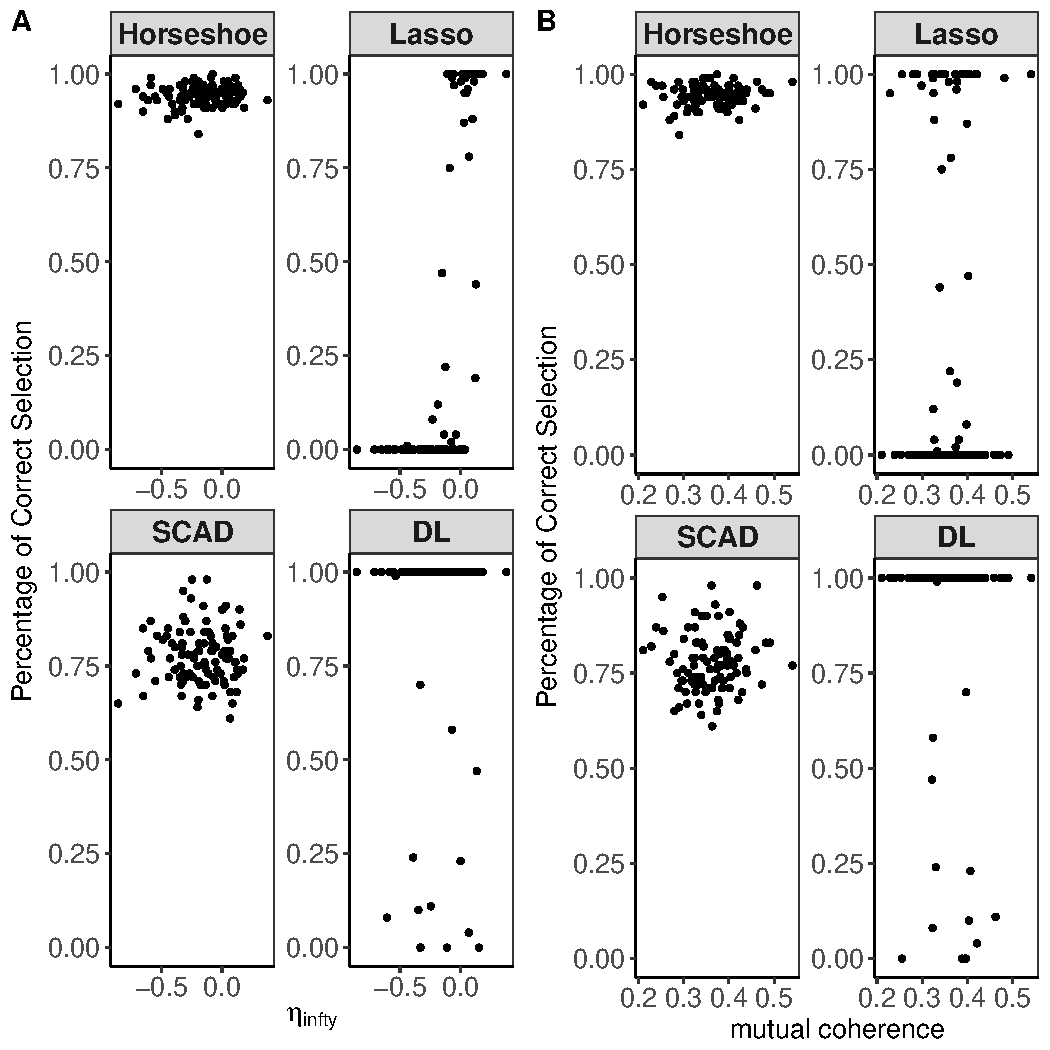
\includegraphics[height = 3in, width=\columnwidth]{irrep_mc_effect_DL_100_100} %height = 3in
\caption{Effect of Strong Irrepresentability Condition $\eta_{\infty}$ and Mutual Coherence
(maximum column correlation) on the percentage of selecting the correct model
by Lasso and SCAD penalty as well as horseshoe and Dirichlet--Laplace (DL) prior.}%
\label{fig:irrep-mc}%
\end{figure}

Figure \ref{fig:irrep-mc} shows the percentage of correctly selected model as a function of the irrepresentable condition number, $\eta_{\infty}$ and mutual coherence  for the four candidates: Lasso, SCAD, horseshoe and Dirichlet--Laplace. For this simulation experiment, Lasso's model selection performance is dependent on the irrepresentability condition, deteriorating with increasing $\eta_{\infty}$. Surprisingly, the effect is weaker for SCAD as well as both the horseshoe and the Dirichlet--Laplace prior. 

While horseshoe almost always recovers the true sparse $\btheta$ vector irrespective of $\eta_{\infty}$, SCAD exhibits a high percentage (mean = $0.75$, range = $[0.61, 0.98]$). Since we have calculated mutual coherence for the same design matrices, in this set-up it does not affect the horseshoe prior's variable selection, and its effect shows no clear pattern on any other candidates. 

\subsection{Binary Response: Logistic Regression}

We compare the performance of horseshoe prior and Lasso for logistic regression for varying degree of dependence between the columns of a design matrix. We generated $n = 100$ binary observation for the standard logistic regression. The true parameter $\btheta^* \in \mathbb{R}^p$ where $p = 32$, $\btheta^*$ is sparse and has 5 non-zero elements $(7, 4, 2, 1, 1)$, and $\sigma^2$ was set to $0.1$. We set the covariance matrix same as the last example, i.e. $\Sigma_{ij} = \rho^{\abs{i-j}}$ and then generate design matrix $\X$ from $\Nor(0, \Sigma)$ for $20$ different values of $\rho \in [0.1, 0.9]$. Since the original horseshoe prior was not designed to handle the logistic likelihood, we use the Gaussian approximation method by \cite{piironen2017sparsity}, where they use a second-order Taylor expansion for the log posterior distribution. \cite{piironen2017sparsity} also propose the regularized horseshoe prior where one introduces an additional slab width $c$ to allow for shrinkage even on the extreme tails. Following the recommendations of \cite{piironen2017sparsity}, we use the regularized horseshoe prior with a hyper-prior $c \sim \text{Inv-Gamma}(2,8)$ that corresponds to a $\text{Student-t}(0, 2^2)$ slab. We use $1,000$ posterior draws per chain with the NUTS algorithm in Stan. For Lasso, we use the \texttt{glmnet} package in R with a $10$-folds cross-validation. 

To compare the two methods for classification and predictive accuracy, we train the models on 80\% of the data, with the remaining as test set and average the results over $50$ random splits. We measure classification accuracy by the number of misclassified response $y_i$'s in test data. For predictive accuracy, we compare the mean log predictive density (MLPD) proposed in \cite{gelman2014understanding} as the mean of the computed log pointwise predictive density, defined as follows. 

Let $\btheta^s$; $s = 1, \ldots, S$ be the posterior draws from $p(\btheta \mid \y)$, and $\y_j$, $j = 1, \ldots, m$ be the $j^{th}$ test data, then MLPD is:

\begin{equation}
\text{MLPD} = \frac{1}{m} \sum_{j=1}^{m} \log \left( \frac{1}{S} \sum_{s=1}^{S} p(\y_j \mid \btheta^s) \right)
\label{eq:mlpd}
\end{equation}

Figure \ref{fig:4a} shows the average number of misclassified observations by horseshoe is a little lower than Lasso for all but two values of $\rho$. For the same values of $\rho$, Fig. \ref{fig:4b} shows that the predictive accuracy under the horseshoe prior is a little better than the Lasso. We direct the readers to \cite{piironen2017sparsity} for a thorough comparison between the different variants of horseshoe prior with Lasso for a few real data set as well as a synthetic data-set with a separable predictor.

\begin{figure}[t!]%
\begin{subfigure}[t]{0.45\linewidth}%
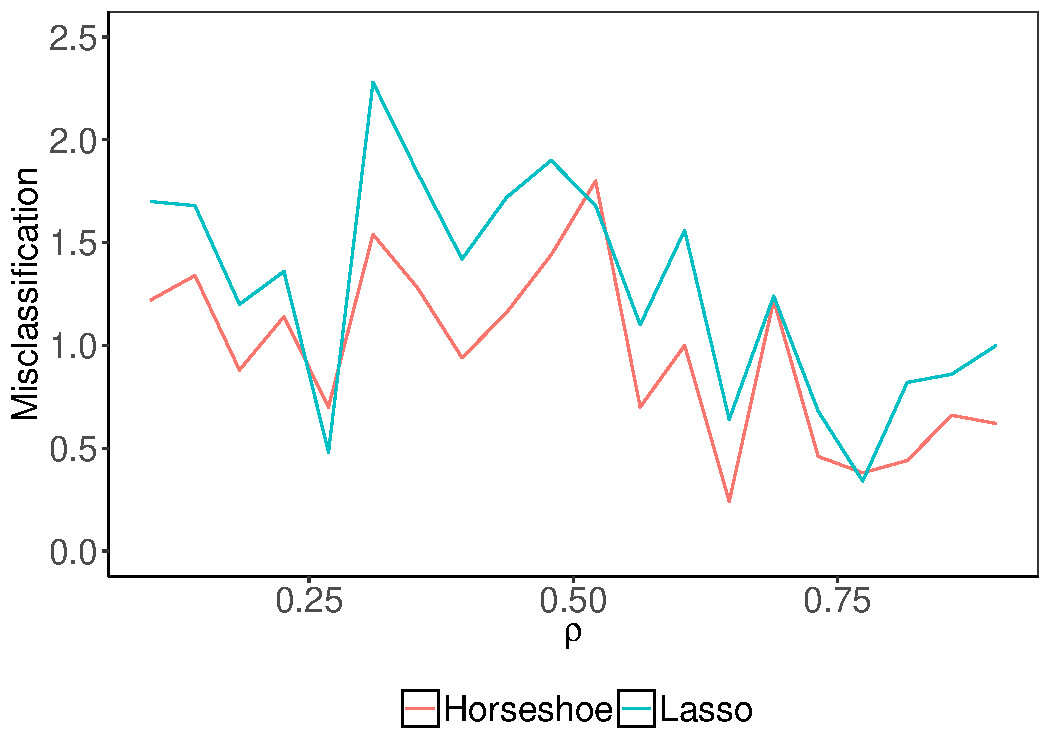
\includegraphics[height=2in,width=\columnwidth]{mp_hs_lasso_20_100_2_ideal_pars}%
%\caption{Number of misclassified test data points}%
\label{fig:4a}%
\end{subfigure}
\begin{subfigure}[t]{0.45\linewidth}%
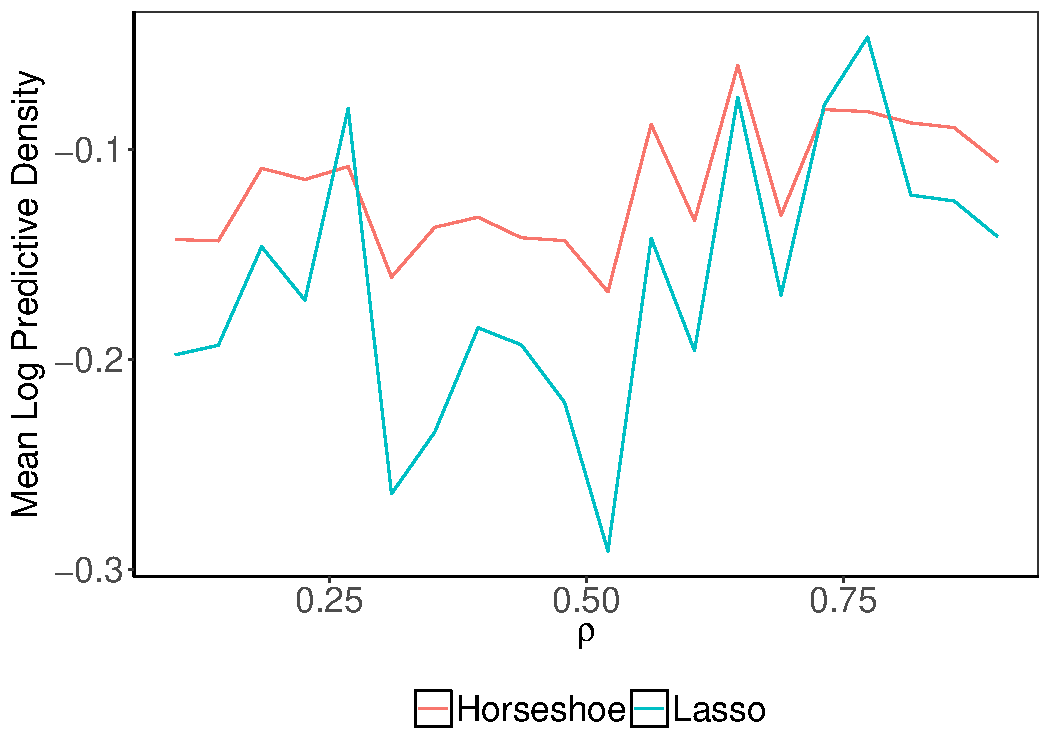
\includegraphics[height=2in,width=\columnwidth]{mlpd_hs_lasso_20_100_2_ideal_pars}%
%\caption{Mean log predictive density in \eqref{eq:mlpd}}%
\label{fig:4b}%
\end{subfigure}
\caption{(a) Number of misclassified test data points and (b) mean log predictive
density in \eqref{eq:mlpd} by the horseshoe and Lasso across different values of correlation
$\rho$: a higher value of $\rho$ represents higher dependence between the columns of $\X$.}%
\label{fig:logistic}%
\end{figure}

\section{Further Developments}\label{sec:app-ext}

%Literature review of applications and extensions and recent development. List papers. 
%Fused and group lasso. Extension to logistic (Polya-Gamma for logistic : MCMC still convex). 

\subsection{Further Developments of Lasso} Since the inception of Lasso as a regularization method for linear regression in 1996, a great deal of extensions and applications have been proposed in the literature. The combined effect of convex penalty and sparsity of the final solution lead to huge computational gains by using powerful convex optimization methods on problems of massive dimensions. The coordinate descent approach \citep{friedman_pathwise_2007, friedman2010regularization} is one particularly promising approach, that works by applying soft-threshold to the least-squares solution obtained on partial residuals, one at a time. The coordinate descent approach is flexible and easy and can be proved to converge to the solution as long as the log-likelihood and penalty are convex \citep{tseng2001convergence}, paving the way for wide applicability of $\ell_1$ penalty in generalized linear models (GLM). The popular R package \texttt{glmnet} provides a nice and easy interface for applying Lasso and elastic-net penalty for a general sparse GLM.

%Although a comprehensive list of regularization methods that extend the idea of %Lasso and even move beyond the convex penalty is beyond the scope of this
%article, we give a list of popular regularization methods in %Table~\ref{tab:lasso:ext}, which is adapted from \citet{tibshirani2014praise}.

\subsection{Further Developments of Horseshoe}

As discussed in Section~\ref{sec:one-gp}, the horseshoe prior belongs to a wider class of global-local shrinkage priors \citep{polson2010shrink} that are characterized by a local shrinkage parameter for recovering large signals and a global shrinkage parameter for adapting to overall sparsity. The class of global-local priors, although differing in their specific goals and design, exhibit some common features: heavy tails for tail-robustness and appreciable mass near zero for sparsity, leading to shared optimality properties. Several authors including \citet{van2015conditions, ghosh2016asymptotic, ghosh2016testing} have provided conditions for optimality of one-group continuous priors for estimation of sparse normal means and multiple testing. 

Although the original horseshoe prior was developed for signal recovery with sparse Gaussian means, the idea of directly modeling the posterior inclusion probability and use of normal-scale mixture to facilitate sparsity is a flexible idea and can be easily generalized to a wider class of problems. \citet{bhadra2015default} show that the horseshoe prior is a good candidate as a default prior for low-dimensional, possibly non-linear functionals of high-dimensional parameter and can resolve long-standing marginalization paradoxes for such problems. \citet{bhadra2016prediction} show how to use global-local priors for prediction and provide theoretical and numerical evidence that it performs better than a variety of competitors including Lasso, ridge, PCR and sparse PLS. 

Moving beyond Gaussianity, \citet{datta2016bayesian} re-discovered the Gauss hypergeometric prior for flexible shrinkage needed for quasi-sparse count data, with a tighter control on false discoveries.
\citet{piironen2016hyperprior} used a Gaussian approximation using a second-order Taylor expansion for the log-likelihood to apply the horseshoe prior for the generalized linear model. \citet{wang2013class} proposed a shrinkage prior based on a scale mixture of uniform for covariance matrix estimation. \citet{peltola2014hierarchical} applies the horseshoe prior for Bayesian linear survival regression for selecting covariates with highest predictive values. A sample of the many applications of horseshoe prior is given in Table \ref{tab:hs-apps}. Given the explosive growth of the methods in
this area, we conjecture that the horseshoe prior would be regarded as a key tool sparse signal recovery and as a default prior for objective Bayesian inference for many important problems. 


% Table generated by Excel2LaTeX from sheet 'Sheet1'
\begin{table}[htbp]
  \centering
  \caption{Applications of the horseshoe prior}
  \footnotesize{
    \begin{tabular}{|p{3in}|p{1.5in}|}
    \hline
    Application  & Authors \bigstrut\\
    \hline
    \textit{Fadeout} method for mean-field variational inference under non-centered parameterizations and stochastic variational inference for undirected graphical model.  & \citet{ingraham_bayesian_2016} \bigstrut[t]\\
    \hline
    Linear regression for Causal inference and Instrumental variable models  & \citet{hahn_shrinkage_2014, hahn_elliptical_2016} \\
    \hline
    Multiclass prediction using DOLDA (Diagonally orthant Latent Dirichlet Allocation)  & \citet{magnusson_dolda_2016} \\
    \hline
    Mendelian Randomization to detect causal effects of interest & \citet{berzuini_mendelian_2016} \\
    \hline 
    Locally adaptive nonparametric curve fitting with shrinkage prior Markov random field (SPMRF) & \citet{faulkner_bayesian_2015} \\
    \hline
    Quasi-Sparse Count Data & \citet{datta2016bayesian} \\
    \hline
    Variable Selection under the projection predictive framework  & \citet{piironen_projection_2015} \bigstrut[b]\\
    \hline
  Dynamic shrinkage Process (dynamic linear model and trend filtering) & \citet{kowal2017dynamic} \\
   \hline 
   Logistic regression with horseshoe prior & \citet{piironen2017sparsity, wei2017bayesian} \\
  \hline  
  Tree ensembles with rule structured horseshoe regularization & \citet{nalenz2017tree} \\
 \hline 
Bayesian compression for deep learning & \citet{louizos2017bayesian} \\
 \hline 
Precision matrix estimation & \citet{li2017graphical} \bigstrut[b]\\
\hline
    \end{tabular}%
    }
  \label{tab:hs-apps}%
\end{table}%


%\begin{enumerate}
%\item \citet{bhadra2015default} use global-local priors in default Bayes Efron problems.
%\item \citet{bhadra2016prediction} show how to use global-local priors for prediction. Performs better than a variety of competitors including lasso, ridge, PCR and sparse PLS.
%\item \citet{datta2015inference} use global-local priors to model the rate parameter for Poisson count data.
%\end{enumerate}


\section{Discussion}\label{sec:9}

Sparsity can be achieved with Lasso and horseshoe regularization, a member of the class of global-local shrinkage priors. The horseshoe prior offers better computational efficiency than the Bayesian two-group priors, while still mimicking the inference and it outperforms the estimator based on Laplace prior, the Bayesian dual of Lasso. The intuitive reason for better performance by the horseshoe prior is its heavy tails and probability spike at zero, which makes it adaptive to sparsity and robust to large signals. A number of computing strategies have been proposed for both the Lasso and the horseshoe prior, based on variants of coordinate descent and MCMC respectively.  We have outlined the distinct algorithmic implementations in \S \ref{sec:horse-comp} and Table~\ref{tab:hs-imp}. Since the goal of Lasso-based estimator is to produce a point estimate, rather than samples from the full posterior distribution of the underlying parameter, Lasso-based methods are typically faster than the horseshoe and related shrinkage priors.

The lack of speed can be overcome easily by employing a strategy based on expectation-maximization or proximal algorithm, which is often faster than the Lasso or other penalty based methods, for example the EM algorithm proposed in \S 4 of \citet{bhadra2017horseshoe} is orders of magnitude than the non-convex SCAD or MCP \citep[\textit{vide} Table 1]{bhadra2017horseshoe}. Another fruitful strategy is to employ proximal algorithms similar to expectation-maximization \citep{polson2015proximal}. These algorithms can be specifically designed to outperform staples such as Lasso \citep{bhadra2017horseshoe} by using clever decompositions of the objective function and some convenient properties (e.g. strong convexity) of the resulting parts. As discussed before, an active area of research is designing algorithms to handle Bayesian shrinkage in big data problems, e.g. using GPU-accelerated computing \citep{terenin_gpu-accelerated_2016}. 

We have discussed the theoretical optimality properties for both Lasso and horseshoe estimator. The optimality properties of Lasso in regression are well-known and they depend on `neighborhood stability' or `irrepresentability' condition \eqref{eq:irrep} and `beta-min' condition. Similarly, adaptive posterior concentration for horseshoe depends on `excessive bias restriction', a condition analogous to `beta-min'. Although horseshoe regression has not been studied to the same depth as penalized regression, it is expected that optimality will depend on conditions that guarantee against ill-posed design matrix and separability of signal and noise parameters. For the sequence model, the horseshoe posterior mean enjoys near-minimaxity in estimation, and the induced decision rule achieves asymptotic Bayes optimality for multiple testing as discussed in Section~\ref{sec:stat-prop}. 

The horseshoe estimator of the sampling density converges to the the true sampling density $p(y \mid \theta_0)$ at a super-efficient rate at $\theta_0 = 0$, compared to any Bayes estimator with a bounded prior density at the origin \citep[\textit{vide} Theorem 4]{carvalho2010horseshoe}. The rate of convergence of the Ces\'aro-average Bayes risk at $\theta_0 = 0$ for horseshoe is $O(n^{-1}(\log n - b \log \log n))$. This is called the `Kullback--Leibler super-efficiency' in true density recovery for the horseshoe estimator. The horseshoe priors are also good default priors for many-to-one functionals as shown in \citet{bhadra2015default}, but a thorough study of horseshoe prior for default Bayes problems is still an unexplored area. 

Global-local shrinkage is still a fruitful area for future research. %For example, the horseshoe prior and related classes can be approached with new computational strategies, such as proximal algorithms \citep{polson2015proximal}. 
We list a few possible directions here. 
\begin{enumerate}
   \item The square-root Lasso \citep{belloni2011square} or scaled Lasso \citep{sun2012scaled} improves over the Lasso by making the inference ambivalent towards $\sigma$, while making the estimator scale-invariant. It might be interesting to study the effect of marginalizing the global parameters such as $\tau$ and $\sigma$ on inference from shrinkage priors. Our preliminary investigation suggests that scaling the prior on $\tau$ by $\sigma$ or marginalizing out $\sigma$ improves the robustness of the shrinkage priors.
	\item One promising area is to extend the inferential capacity for the exponential family, and whether or not the optimality properties carry over to the non-Gaussian cases. Some early research on this is \citet{datta2016bayesian} and \citet{wei2017bayesian}. 
	\item Another interesting direction could include structured sparsity under the horseshoe prior, such as grouped variable selection and Gaussian graphical models, as explored in \cite{li2017graphical}. 
\end{enumerate}
%\textcolor{red}{
%What's left to do? Horseshoe subset selection. Lasso computationally quick / scalable. Horseshoe needs MCMC etc. 
%\begin{enumerate}
%\item So many global-local priors; what is the unifying theme? Spike and heavy tails \citet{polson2010shrink,van2015conditions}.
%\item How close to minimax constant can we get in estimation? Only near-minimaxity and the best constant is $4\sigma^2$ \citep{van2017adaptive}.
%\item How close to oracle risk can we get in testing? We can get exact rate \citep{ghosh2016testing}.
%\item Is prediction performance optimal? 
%\item Yet to rigorously show global-local priors have any information theoretic properties in default Bayes problems that reference priors \citep{berger_development_1992} enjoy.
%\item \citet{bhadra2016global} demonstrate how global-local mixtures can be generated using two integral identities. This might prove useful in EM and MCMC.
%\end{enumerate}
%}

\begin{appendix}

%\section{Appendix: Algorithms}

%Literature review of algorithms and R packages. 
%LASSO: glmnet, genlasso. 
%Horseshoe: horseshoe, fastHorseshoe, monomvn, our own package. 

%\section*{Appendix}
%Possibly give some R code vignette.

%\section*{Other refs}
%The 1988 Neyman Memorial Lecture: A Galtonian Perspective on Shrinkage Estimators - Stephen M. Stigler

\section{Two-groups Model}\label{sec:2gp}

The two-groups model is a natural hierarchical Bayesian model for the sparse
signal-recovery problem.  The two-groups solution to the signal detection
problem is as follows:
\begin{enumerate}
\item Assume each $\theta_i$ is non-zero with some common prior probability $(1 - \pi)$, and that the nonzero $\theta_i$ come from a common density $\Nor(0,\psi^2)$. 
\item Calculate the posterior probabilities that each $y_i$ comes from $\Nor(0,\psi^2)$. 
\end{enumerate}
The most important aspect of this model is that it automatically adjusts for multiplicity without any ad-hoc regularization, i.e. it lets the data choose $\pi$ and then carry out the tests on the basis of the posterior inclusion probabilities $\omega_i = P(\theta_i \neq 0 \mid y_i)$. Formally, in a two-groups model $\theta_i$'s are modeled as

\begin{equation}
\theta_i \mid \pi, \psi = (1-\pi)\delta_{0} + \pi \Nor (0, \psi^2), \label{spikeslab}
\end{equation}

where $\delta_{0}$ denotes a point mass at zero and the parameter $\psi^2>0$ is
the non-centrality parameter that determines the separation between the two
groups. Under these assumptions, the marginal distribution of $(y_i \mid \pi, \psi)$
is given by:

\begin{equation}
y_i \mid \pi, \psi \sim  (1-\pi) \Nor(0, 1) + \pi \Nor(0, 1+\psi^2). \label{twogroups}
\end{equation}

%For the theoretical discussion, we will confine ourselves to the case where $\sigma_0^2 = 1$, a common assumption for multiple testing asymptotics (see Abramovich et al. (2006) and \cite{bogdan2008comparison,bogdan2011asymptotic} for example). 
From \eqref{twogroups}, we see that the two-groups model leads to a sparse
estimate, i.e., it puts exact zeros in the model. 

\section{Proof of Equation (3.6)}\label{sec:proof}

Assume $\sigma^2 = 1$ without loss of generality. The hierarchical model for horseshoe prior is $y_i \sim \Nor(\theta_i,1)$ and $\theta_i \sim \Nor(0, \lambda_i^2 \tau^2)$. Using Bayes' rule, posterior density of $\theta_i$ is Gaussian with mean $(1-\kappa_i)y_i$ where $\kappa_i = 1 / (1 + \lambda_i^2 \tau^2)$. It follows from Fubini's theorem:
\[
E(\theta_i \mid y_i) = \int_0^1 (1-\kappa_i)y_i p(\kappa_i \mid y_i) d \kappa_i = \{1 - E(\kappa_i \mid y_i)\} y_i 
\]

\section{Shrinkage Profiles}\label{sec:shrink}
We compare the shrinkage functions for Lasso, ridge, and the horseshoe estimator with that of the post-lava estimator \citep{chernozhukov2017lava}. The shrinkage functions for these methods are given below:

\begin{align}
d_{\text{lasso}}(z) & = \argmin_{\theta \in \mathbb{R}} \{ (z-\theta)^2 + \lambda_l \abs{\theta} \} = (\abs{z} - \lambda_l/2)_{+} sgn(z) \\
d_{\text{ridge}}(z) & = \argmin_{\theta \in \mathbb{R}} \{ (z-\theta)^2 + \lambda_r \theta^2 \}= (1 + \lambda_r)^{-1} z \\
d_{\text{post-lava}}(z) & = \begin{cases} 
                                         z & \quad \abs{z} > \lambda_1/2k \\
                                         (1-k)z & \quad \abs{z} \le \lambda_1/2k,
                                        \end{cases}
\; \text{where} \; k = \lambda_2/ (1 + \lambda_2) \\
d_{\text{horseshoe}}(z) & = z \left( 1 - \frac{2 \Phi_1(1/2,1,5/2,z^2/2,1-1/\tau^2)}{3\Phi_1(1/2,1,3/2, z^2/2, 1 - 1/\tau^2)} \right) 
\end{align}

Figure \ref{fig:score} shows the post-lava and the horseshoe shrinkage function along with Lasso and ridge shrinkage functions for $z > 0$. Although a theoretical analysis is beyond the scope of the current article, we can see the similarities between the lava and horseshoe shrinkage. They both shrink aggressively for small values of $z$ and provide robustness for large signals $z$, as the shrinkage function becomes closer to the $45^\circ$ line.
\end{appendix}

\section*{Acknowledgements}
We thank the AE and two anonymous referees for constructive suggestions. Bhadra and Polson are partially supported by Grant No. DMS-1613063 by the US National Science Foundation.

\bibliographystyle{authordate1}
\bibliography{hs-review}

\end{document}